\documentclass[12pt, a4paper]{book}
\begin{document}
\chapter{Results}\label{chap:results}
The time has come to test how our networks fare on learning our models. This chapter showcases the results of boths methods we used. The first method, which we called the model dependent approach, which trains one BDT for each model we have, including all the mass points and simulated samples. 
And the second method, which we called the model independent approach, where we split the dataset in orthogonal Signal Regions (SR). The regions we studied are
\begin{itemize}
   \item SR1: $m_{ll} >110$ GeV and $E_T^{miss} \in [50, 100]$ GeV
   \item SR2: $m_{ll} >110$ GeV and $E_T^{miss} \in [100, 150]$ GeV
   \item SR3: $m_{ll} >110$ GeV and $E_T^{miss} >150$ GeV
\end{itemize}
To test how well the networks have learned the models we will create a mass exclusion limits for every model. We decided to make a cut of $m_{ll} >110$ GeV for the mono-Z' models when using the model dependent approach to reduce computational time.\\
\\To compare the last method to the first we will statistically combine the mass exclusions results for each SR for each final state in a model. To navigate through the process we will look at the Dark Higgs Heavy Dark Sector model, using the model dependent method, 
as the model independent method does the same with three SRs. Afterwards we will present the combined exclusion limits for every model for both methods.


\graphicspath{{../../../Plots/}}
\section{Walkthrough of method}\label{sec:Walkthrough}
We conducted a grid search to optimize the BDT and trained the network using 80\% of the SM background samples and 80\% of every different $Z'$ mass sample of the model. Using this approach for this model gave the features in Figure \ref{fig:DH_HDS_feat} as the most important ones. The most important variables here are the ones which we expect 
to be important on a dilepton and MET final state.\\
\begin{figure}[!ht]
	\centering
      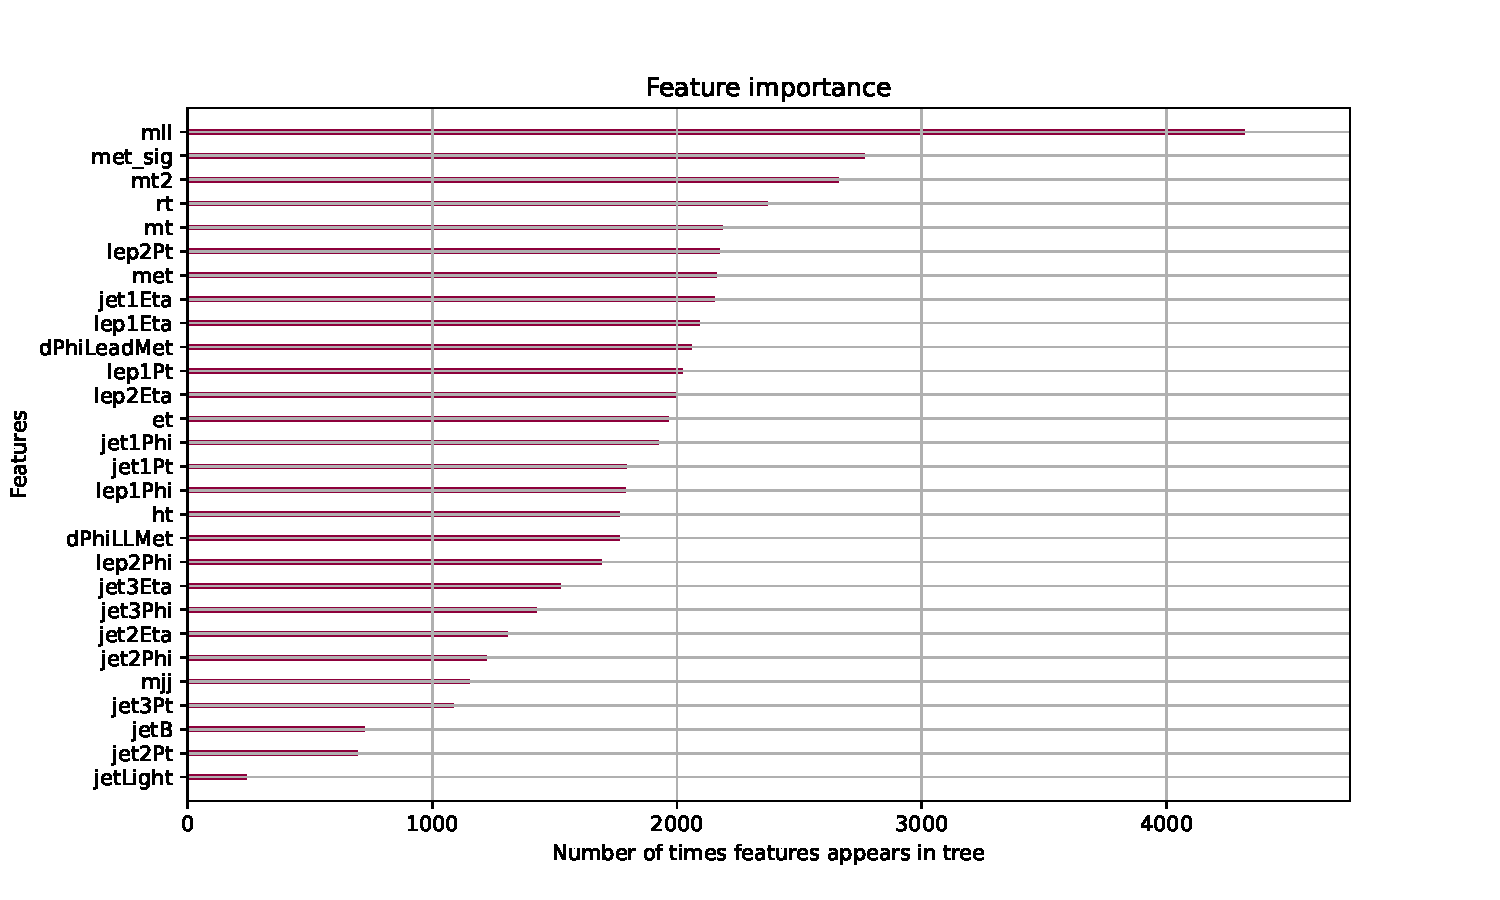
\includegraphics[width=0.75\textwidth]{XGBoost/DH_HDS/feature_importance/weight.pdf}
   \caption{Feature importance for network trained on Z' DH HDS using the weight metric. To see the feature importance plots with the other metrics see Appendix \ref{apx:MDA}.}\label{fig:DH_HDS_feat}
\end{figure}
\\To showcase how the network sorts signal from background we can see the validation plots in Figure \ref{fig:DH_HDS_vals} showing some of the signal samples.\\
\begin{figure}[!ht]
	\centering
	\begin{subfigure}[b]{0.49\textwidth}
      \centering
      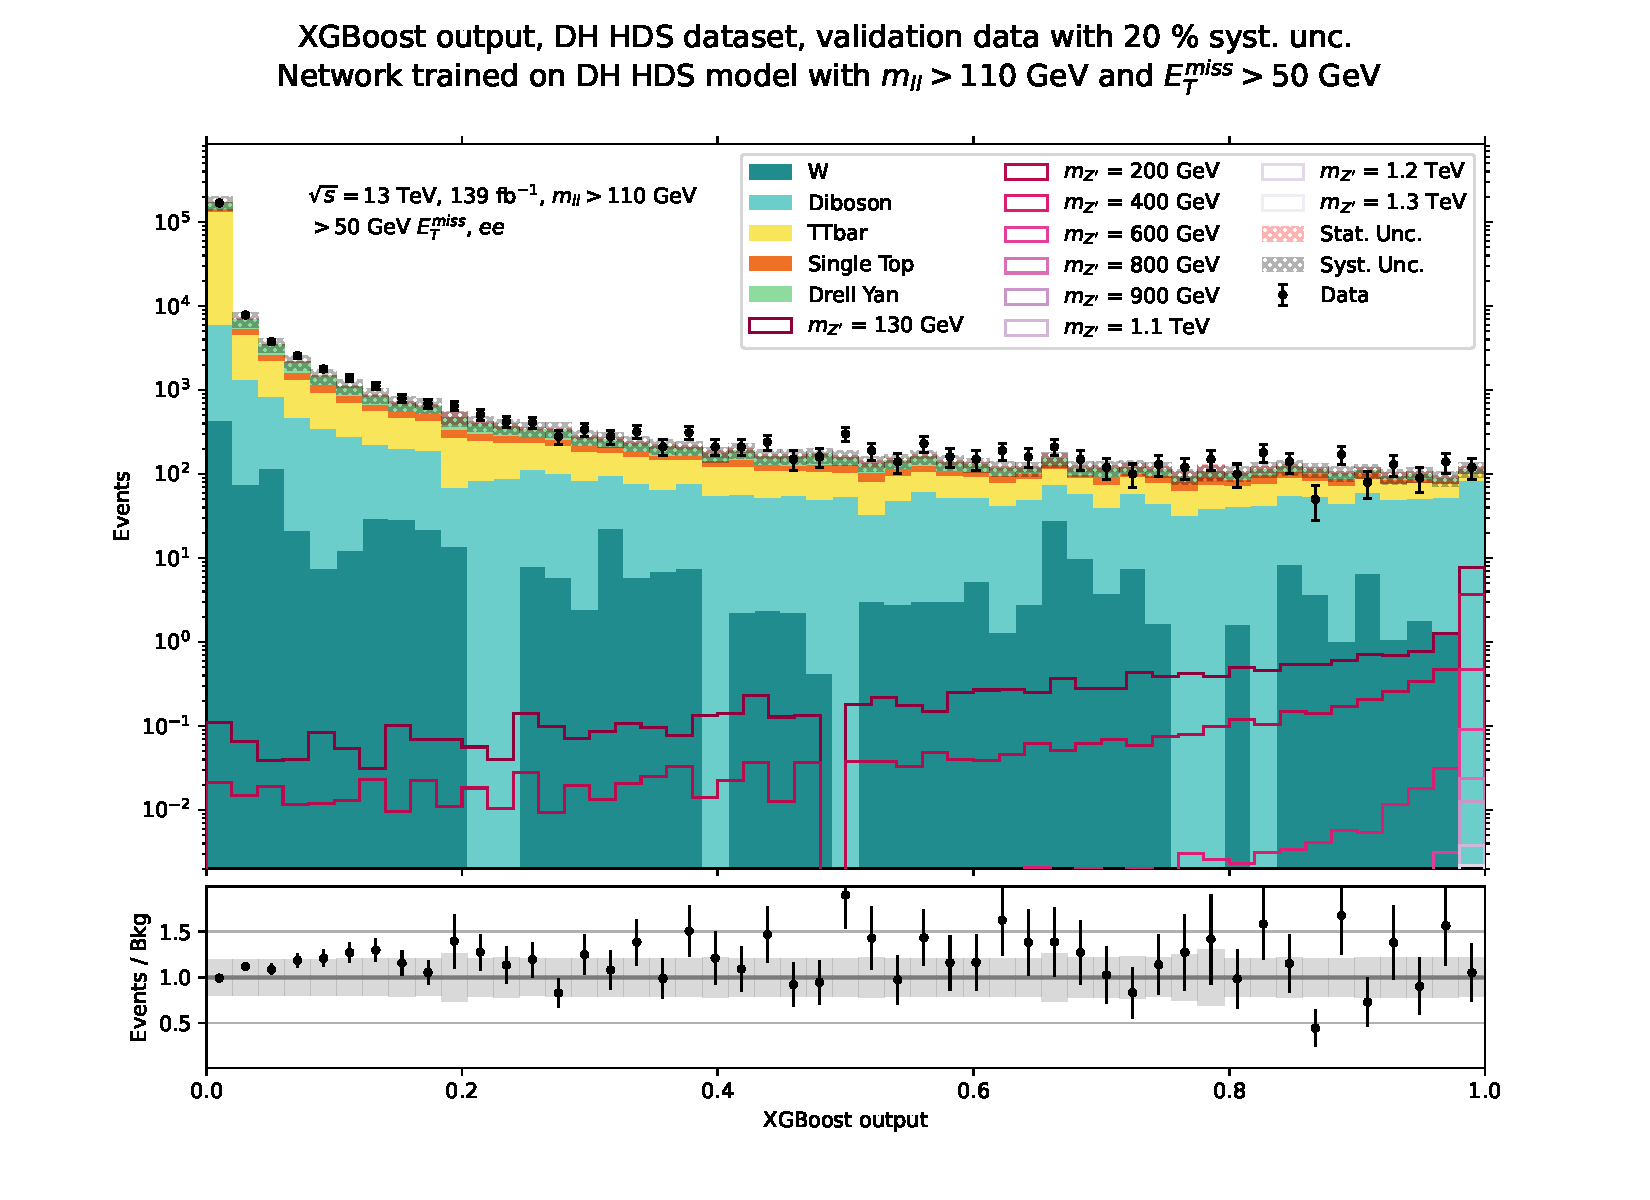
\includegraphics[width=1\textwidth]{XGBoost/DH_HDS/VAL_ee.pdf}
      \end{subfigure}
   \hfill
   \begin{subfigure}[b]{0.49\textwidth}
      \centering
      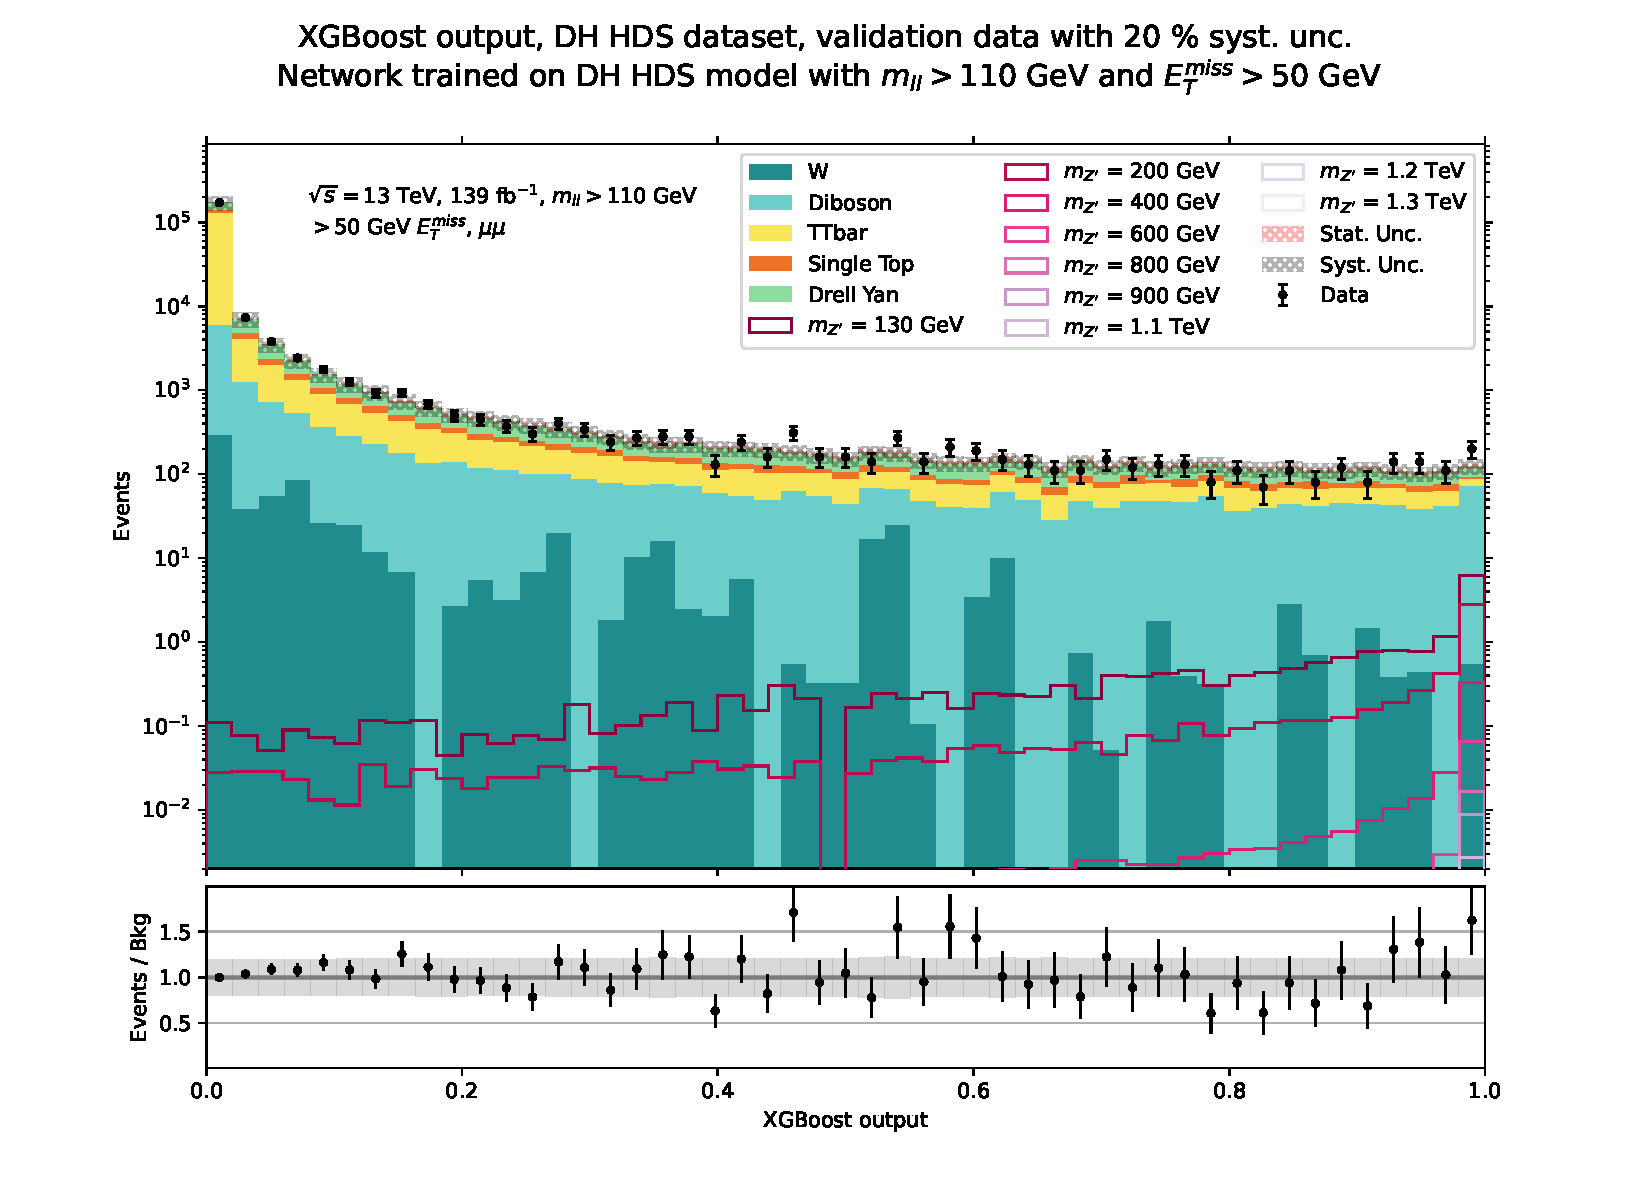
\includegraphics[width=1\textwidth]{XGBoost/DH_HDS/VAL_uu.pdf}
      \end{subfigure}
   \caption{Validation plots for network trained on Z' DH HDS}\label{fig:DH_HDS_vals}
\end{figure}
\\While the validation plot might indicate that the network is not doing an impressive job at sorting signal from background, we can actually see how well the network learns the different mass points by looking at the ROC curves for each mass point, this is shown in Figure \ref{fig:DH_HDS_ROCS}. 
Here we see that the network struggles a tiny bit to learn the models with lowest $m_{Z'}$, but the AUC score is still 0.96, meaning that it actually learned to sort the signal from SM background.\\
\begin{figure}[!ht]
	\centering
	\begin{subfigure}[b]{0.49\textwidth}
      \centering
      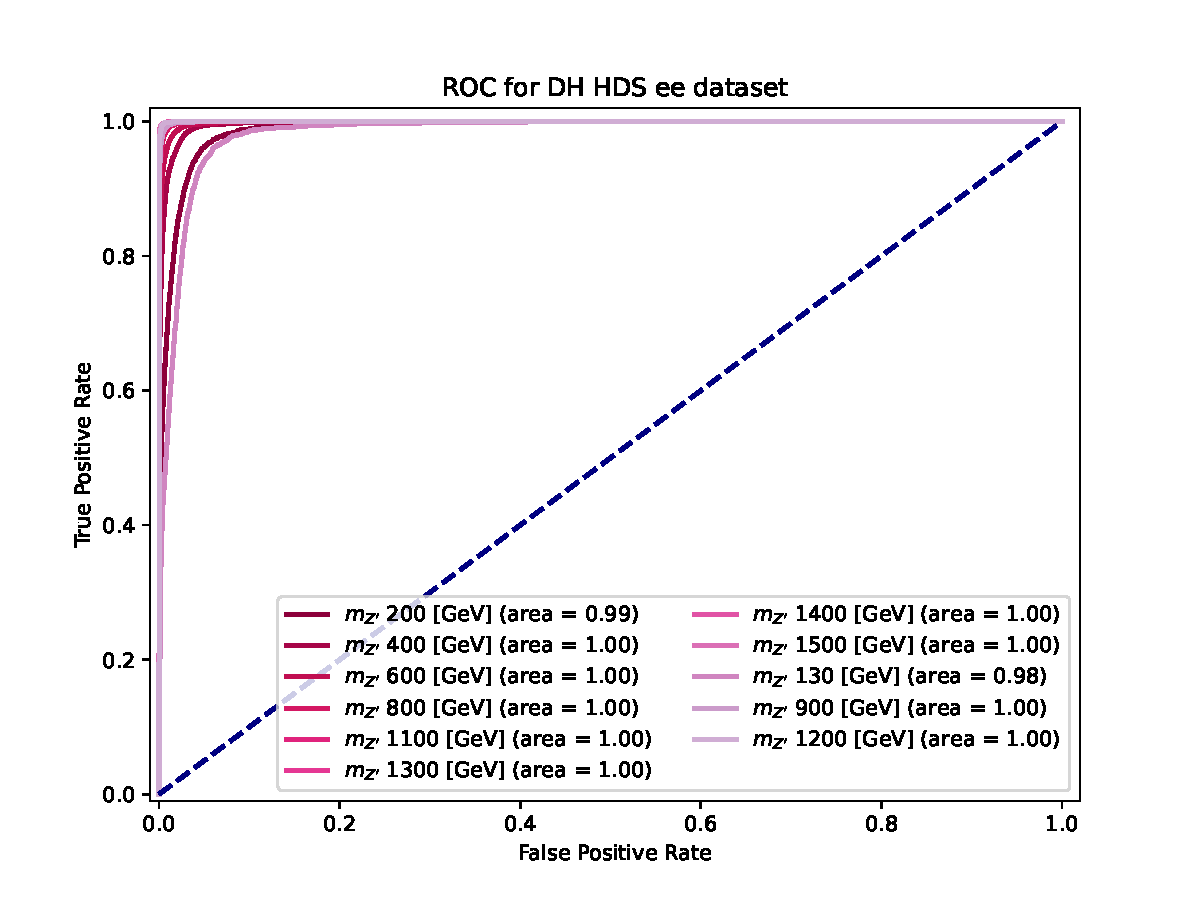
\includegraphics[width=1\textwidth]{XGBoost/DH_HDS/ROC_ee.pdf}
      \end{subfigure}
   \hfill
   \begin{subfigure}[b]{0.49\textwidth}
      \centering
      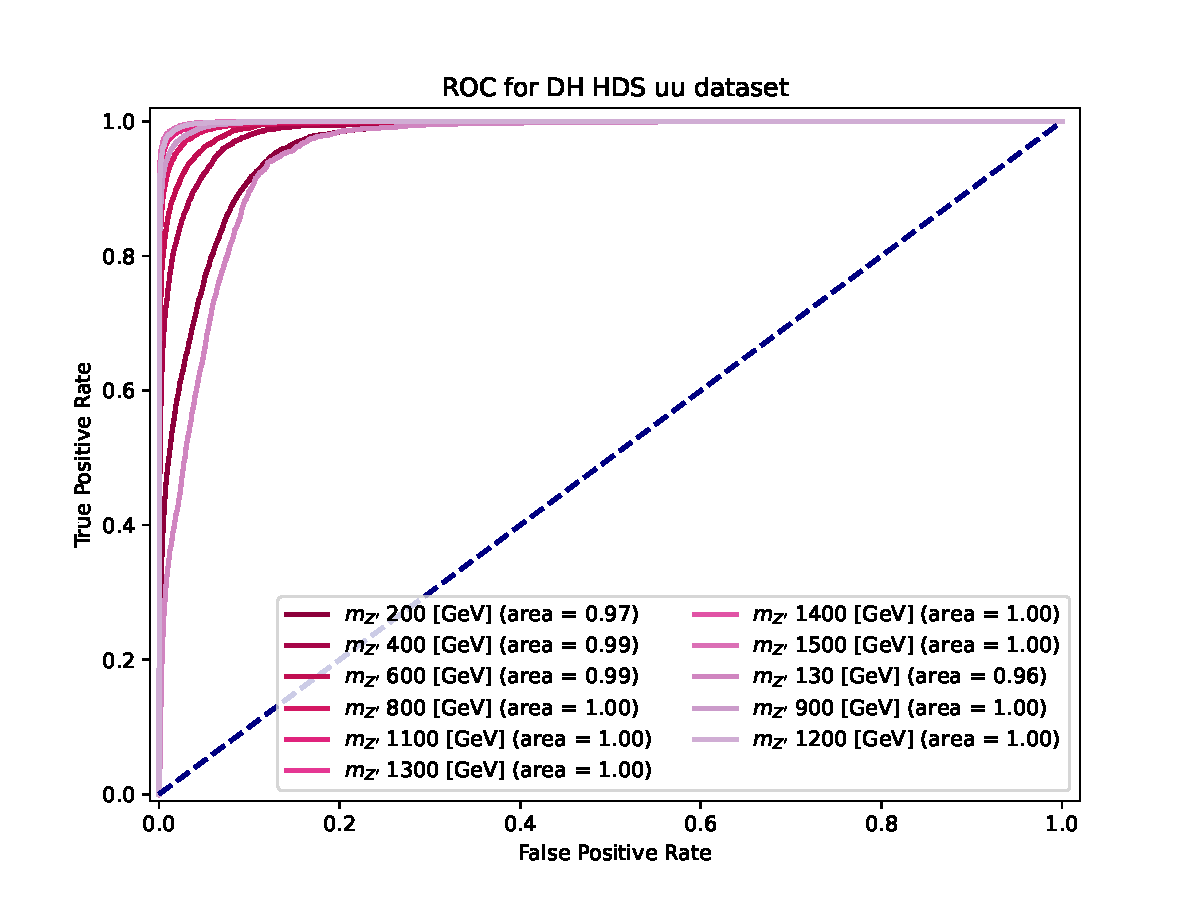
\includegraphics[width=1\textwidth]{XGBoost/DH_HDS/ROC_uu.pdf}
      \end{subfigure}
   \caption{ROC plots for every Z' mass point on network trained on Z' DH HDS}\label{fig:DH_HDS_ROCS}
\end{figure}
\\To define the region we will use to make any exclusions we can choose the validation plot bin that gives us the highest significance, this can be seen in Figure \ref{fig:DH_HDS_exp_sig} for a few mass points. From this we see that we get the best expected significance 
of approximately 0.7$\sigma$ (without uncertainties), even though the network got an AUC score of 0.96 for the mass point on the muon channel. From this we see that even with an AUC of 0.96 we do not manage to exclude the model.\\
\begin{figure}[!ht]
	\centering
	\begin{subfigure}[b]{0.49\textwidth}
      \centering
      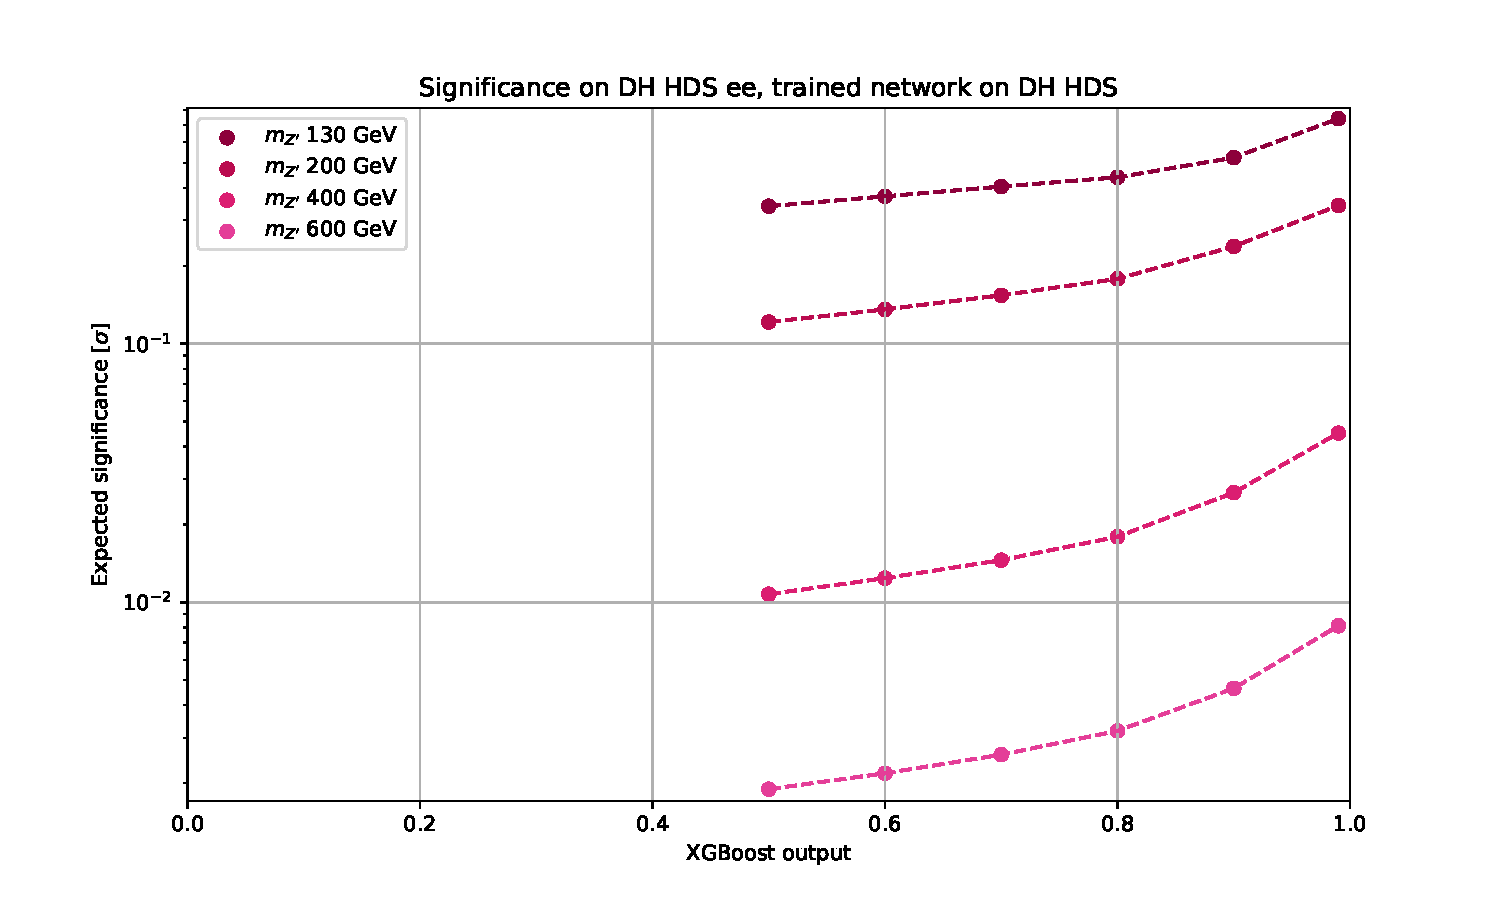
\includegraphics[width=1\textwidth]{XGBoost/DH_HDS/EXP_SIG_ee.pdf}
      \end{subfigure}
   \hfill
   \begin{subfigure}[b]{0.49\textwidth}
      \centering
      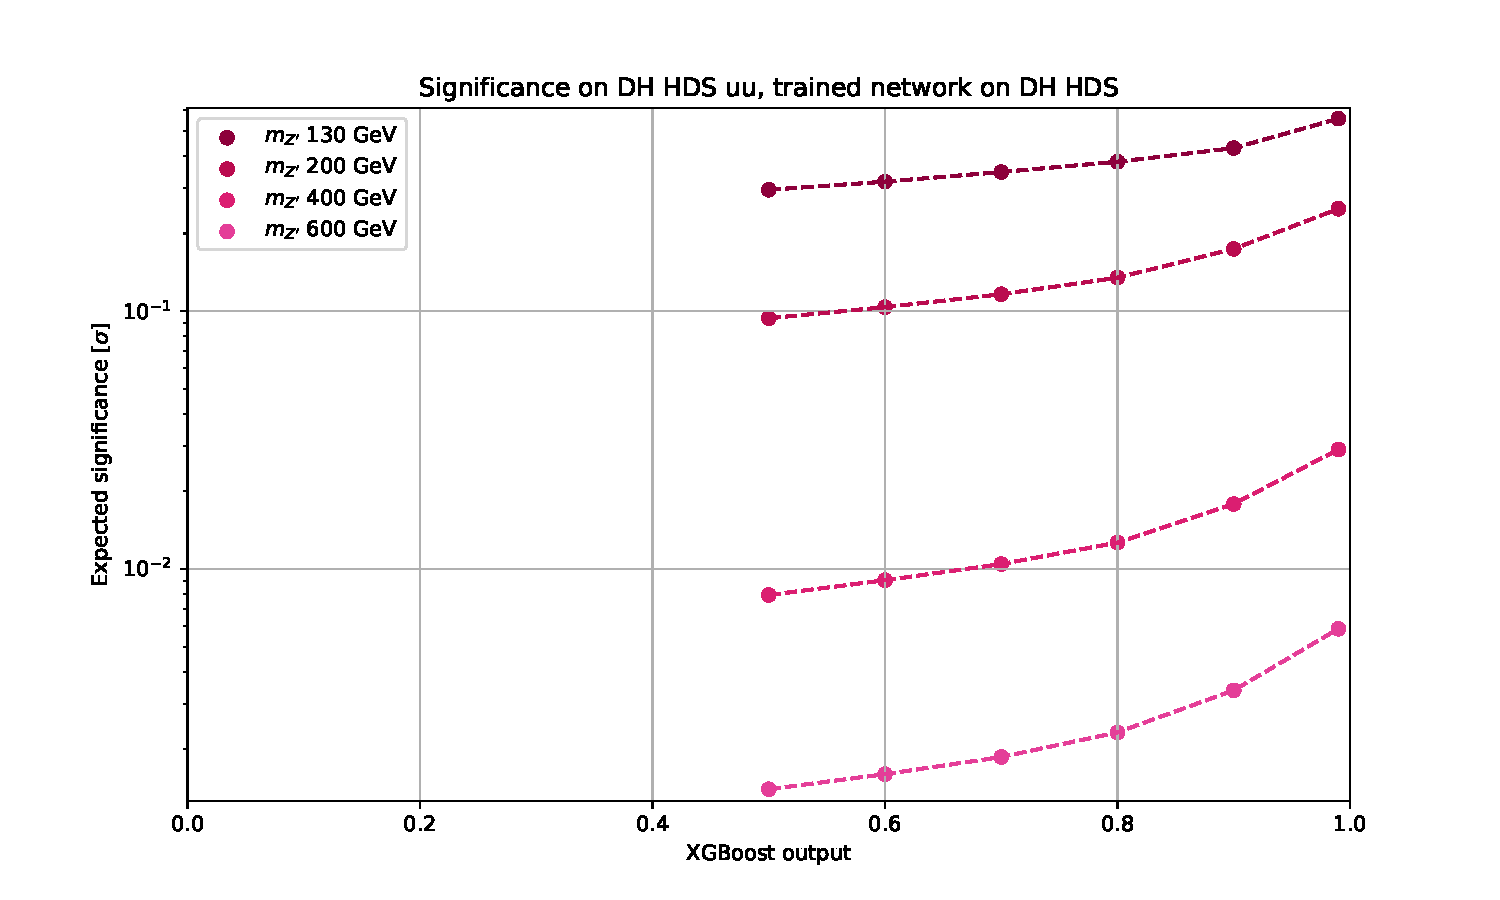
\includegraphics[width=1\textwidth]{XGBoost/DH_HDS/EXP_SIG_uu.pdf}
      \end{subfigure}
   \caption{Expected significance plots for Z' mass points on network trained on Z' DH HDS}\label{fig:DH_HDS_exp_sig}
\end{figure}
\\As the last bin has the greatest significance, we can effectively make a cut based on the BDT score. Counting the number of events on this last bin, as well as their uncertainties we can calculate a mass exclusion for both electron and muon channel. 
Following the method explained in Chapter \ref{sec:stat_anal} using the $\varepsilon_{\text{sig}}$, $N_{\text{bkg}}$ and $\sigma B$ from Table \ref{tab:stat_vals_DH_HDS} we can create a mass exclusion for each leptonic channel. 
\begin{table}[!ht]\centering\caption[Inputs for the $Z'h_D\rightarrow l^+l^-\chi\chi$ HDS $\sigma B$ calculations]{Inputs for the $Z'h_D\rightarrow l^+l^-\chi\chi$ HDS $\sigma B$ calculations. The first three columns are the $Z'$ mass, the theoretical cross-section times branching ratio $\sigma B$, and what $Z'$ decay channel we are looking at. 
   The next two are $\varepsilon_{\text{sig}}$, which is the signal selection efficiency, and $N_{\text{sig}}$, which is the theoretical number of signal events after the cuts. The last two columns are the number of background events, $N_{\text{bkg}}$, 
   and the events observed in the data, $N_{\text{obs}}$. The uncertainties of $\varepsilon_{\text{sig}}$, $N_{\text{sig}}$ and $N_{\text{bkg}}$ are statistical with an assumed 20\% systematic uncertainty. The MET threshold is $E_{\text{T,min}}^{\text{miss}}=50$GeV and the invariant mass threshold is $m_{ll}^{min}=110$GeV 
   and is the same for all inputs.}
   \small\begin{tabular}{@{}ccc|ccc@{}}
      \midrule\midrule 
         $m_{Z'}$ [GeV] & $\sigma B$ [fb] & Channel & $\varepsilon_{\text{sig}}$ $[\times10^{-1}]$& $N_{\text{sig}}$ & $N_{\text{bkg}}$ \\\midrule\midrule
         \multirow{2}{*}[-2\baselineskip]{130}& \multirow{2}{*}[-2\baselineskip]{$1.11$}& $ee$ & $0.25\pm0.05$ & $7.80\pm1.58$ & $108.4\pm23.0$ \\ 
         & & $\mu\mu$ & $0.20\pm0.04$ & $6.28\pm1.27$ & $124.9\pm26.1$ \\ \midrule
         \multirow{2}{*}[-2\baselineskip]{200}& \multirow{2}{*}[-2\baselineskip]{$2.46\times10^{-1}$}& $ee$ & $0.54\pm0.11$ & $3.67\pm0.74$ & $114.1\pm24.4$ \\ 
         & & $\mu\mu$ & $0.41\pm0.08$ & $2.78\pm0.56$ & $123.2\pm25.8$ \\ \midrule
         \multirow{2}{*}[-2\baselineskip]{400}& \multirow{2}{*}[-2\baselineskip]{$1.49\times10^{-2}$}& $ee$ & $1.13\pm0.23$ & $4.67\times10^{-1}\pm9.37\times10^{-2}$ & $107.0\pm23.4$ \\ 
         & & $\mu\mu$ & $0.79\pm0.16$ & $3.29\times10^{-1}\pm6.60\times10^{-2}$ & $127.5\pm26.6$ \\ \midrule
         \multirow{2}{*}[-2\baselineskip]{600}& \multirow{2}{*}[-2\baselineskip]{$2.35\times10^{-3}$}& $ee$ & $1.40\pm0.28$ & $9.12\times10^{-2}\pm1.83\times10^{-2}$ & $126.3\pm26.7$ \\ 
         & & $\mu\mu$ & $1.01\pm0.20$ & $6.59\times10^{-2}\pm1.32\times10^{-2}$ & $126.3\pm26.3$ \\ \midrule
         \multirow{2}{*}[-2\baselineskip]{800}& \multirow{2}{*}[-2\baselineskip]{$5.43\times10^{-4}$}& $ee$ & $1.59\pm0.32$ & $2.40\times10^{-2}\pm4.81\times10^{-3}$ & $118.8\pm25.6$ \\ 
         & & $\mu\mu$ & $1.11\pm0.22$ & $1.67\times10^{-2}\pm3.36\times10^{-3}$ & $113.2\pm23.6$ \\ \midrule
         \multirow{2}{*}[-2\baselineskip]{900}& \multirow{2}{*}[-2\baselineskip]{$2.82\times10^{-4}$}& $ee$ & $1.60\pm0.32$ & $1.25\times10^{-2}\pm2.51\times10^{-3}$ & $119.3\pm25.7$ \\ 
         & & $\mu\mu$ & $1.12\pm0.22$ & $8.78\times10^{-3}\pm1.76\times10^{-3}$ & $114.8\pm24.0$ \\ \midrule
         \multirow{2}{*}[-2\baselineskip]{1100}& \multirow{2}{*}[-2\baselineskip]{$8.40\times10^{-5}$}& $ee$ & $1.63\pm0.33$ & $3.81\times10^{-3}\pm7.64\times10^{-4}$ & $114.3\pm24.4$ \\ 
         & & $\mu\mu$ & $1.16\pm0.23$ & $2.70\times10^{-3}\pm5.42\times10^{-4}$ & $118.6\pm24.7$ \\ \midrule
         \multirow{2}{*}[-2\baselineskip]{1200}& \multirow{2}{*}[-2\baselineskip]{$4.75\times10^{-5}$}& $ee$ & $1.65\pm0.33$ & $2.18\times10^{-3}\pm4.37\times10^{-4}$ & $118.4\pm25.1$ \\ 
         & & $\mu\mu$ & $1.14\pm0.23$ & $1.50\times10^{-3}\pm3.01\times10^{-4}$ & $125.6\pm26.3$ \\ \midrule
         \multirow{2}{*}[-2\baselineskip]{1300}& \multirow{2}{*}[-2\baselineskip]{$2.73\times10^{-5}$}& $ee$ & $1.69\pm0.34$ & $1.28\times10^{-3}\pm2.57\times10^{-4}$ & $123.9\pm26.5$ \\ 
         & & $\mu\mu$ & $1.15\pm0.23$ & $8.72\times10^{-4}\pm1.75\times10^{-4}$ & $130.7\pm27.2$ \\ \midrule
         \multirow{2}{*}[-2\baselineskip]{1400}& \multirow{2}{*}[-2\baselineskip]{$1.60\times10^{-5}$}& $ee$ & $1.67\pm0.33$ & $7.43\times10^{-4}\pm1.49\times10^{-4}$ & $115.8\pm24.5$ \\ 
         & & $\mu\mu$ & $1.16\pm0.23$ & $5.15\times10^{-4}\pm1.03\times10^{-4}$ & $125.4\pm26.1$ \\ \midrule
         \multirow{2}{*}[-2\baselineskip]{1500}& \multirow{2}{*}[-2\baselineskip]{$9.42\times10^{-6}$}& $ee$ & $1.69\pm0.34$ & $4.44\times10^{-4}\pm8.90\times10^{-5}$ & $123.9\pm26.5$ \\ 
         & & $\mu\mu$ & $1.13\pm0.23$ & $2.97\times10^{-4}\pm5.96\times10^{-5}$ & $130.7\pm27.2$ \\
      \midrule\midrule
   \end{tabular}
   \label{tab:stat_vals_DH_HDS}
\end{table}
The results can be seen in Figure \ref{fig:DH_HDS_exclusion_ee_uu}.
\clearpage
\begin{figure}[!ht]
	\centering
   \begin{subfigure}[b]{0.49\textwidth}
      \centering
      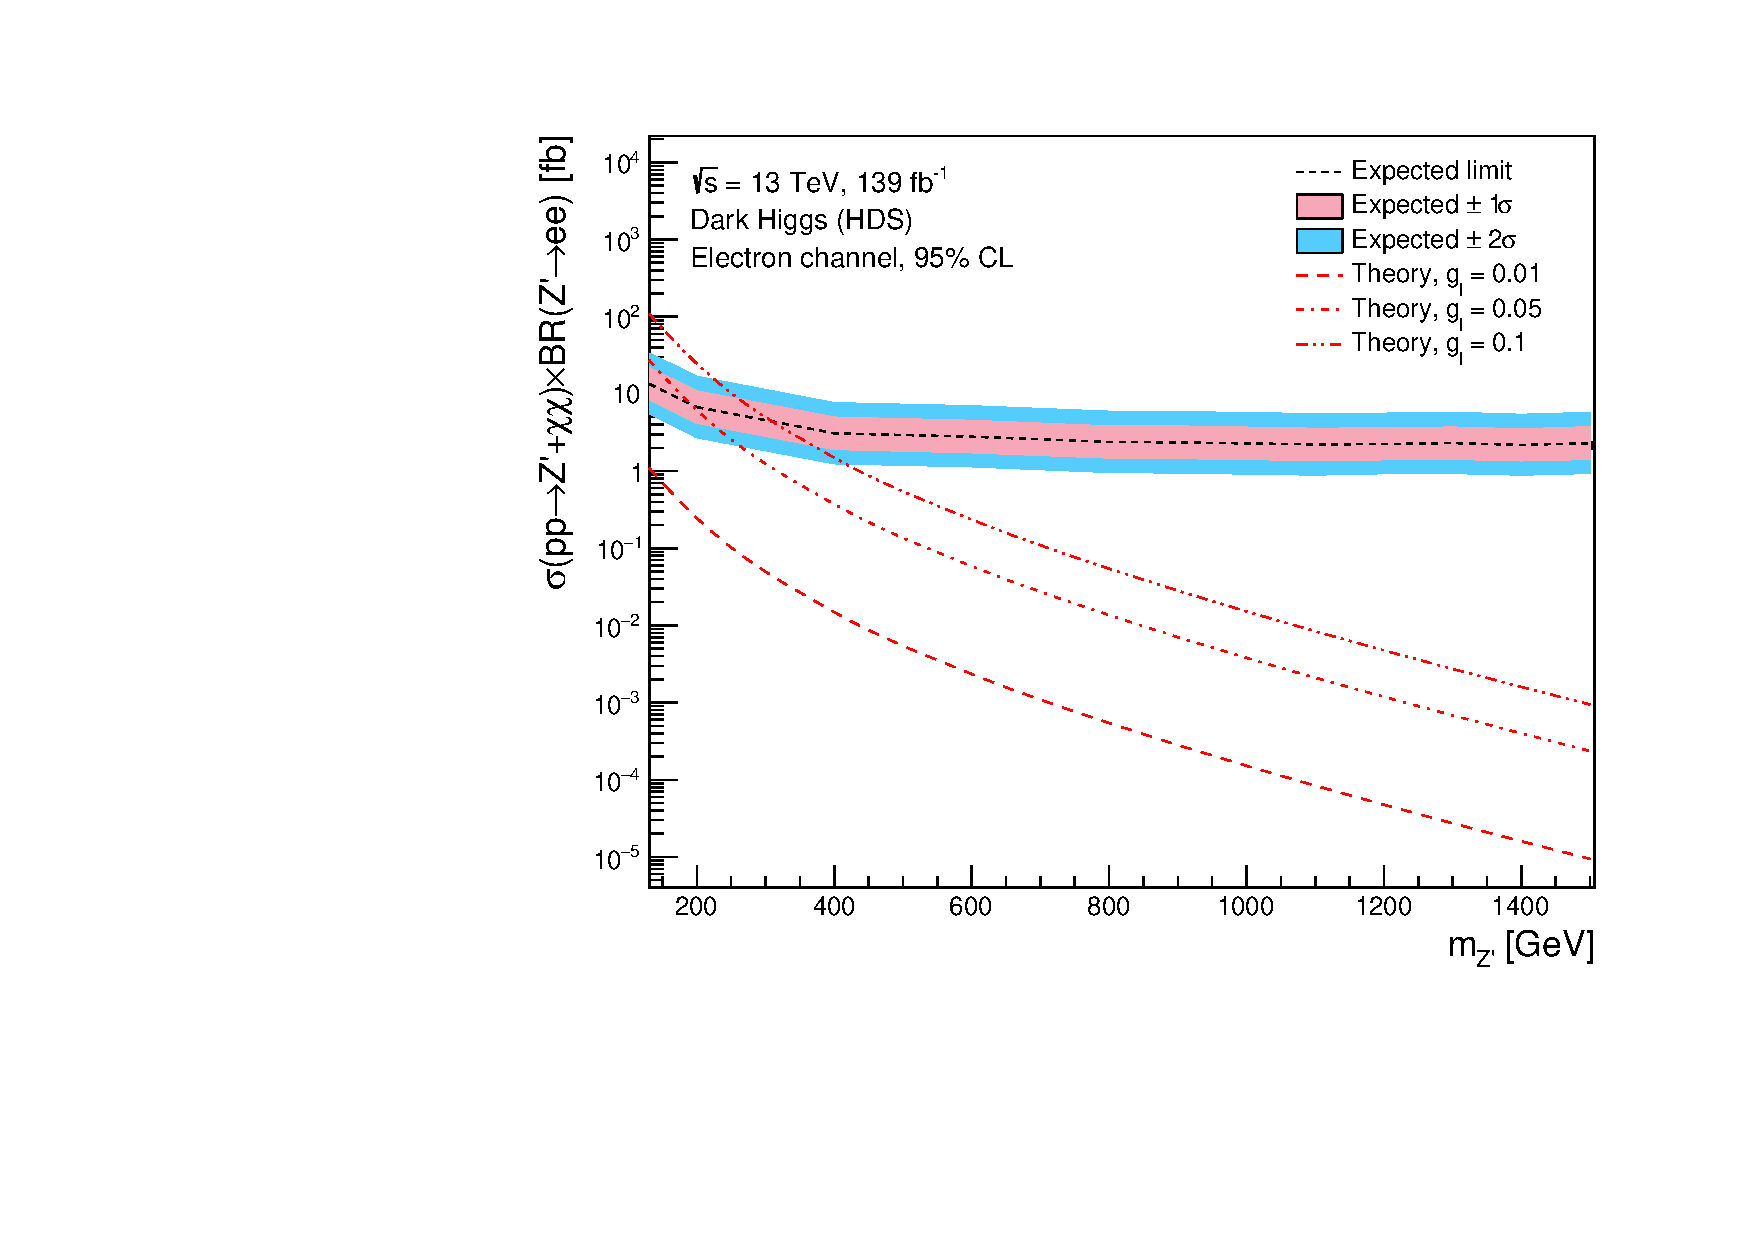
\includegraphics[width=1\textwidth]{Limits/DH_HDS/mass_exclusion_ee.pdf}
      \end{subfigure}
   \hfill
   \begin{subfigure}[b]{0.49\textwidth}
      \centering
      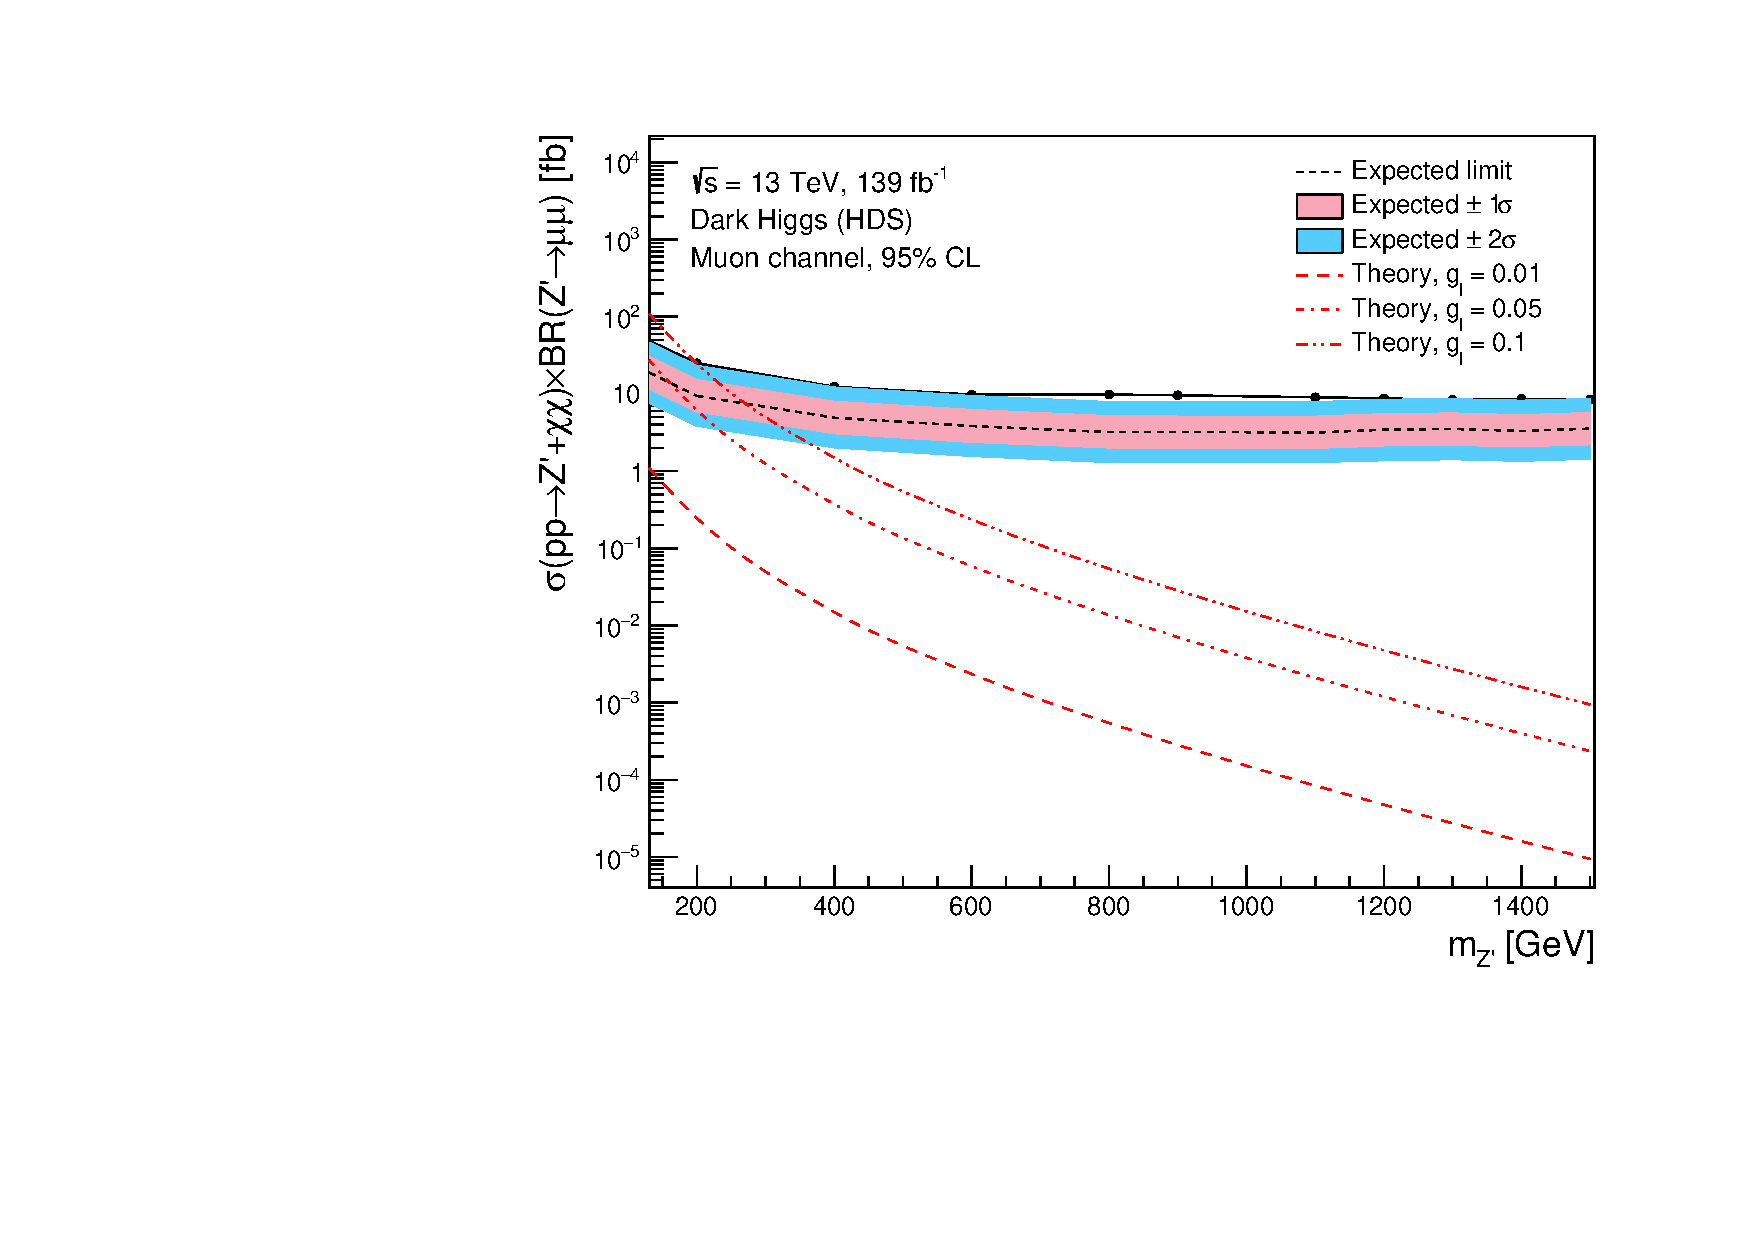
\includegraphics[width=1\textwidth]{Limits/DH_HDS/mass_exclusion_uu.pdf}
      \end{subfigure}
   \caption{Mass exclusion limits of $ee$ and $\mu\mu$ channel for all Z' DH HDS model}\label{fig:DH_HDS_exclusion_ee_uu}
\end{figure}
\noindent We can furthermore statistically combine both of these results to get the exclusion on a general dilepton final state. Following this method for all other five models\footnote{For more plots look at the GitHub repo: in \href{https://github.com/rubenguevara/Master-Thesis/tree/master/Plots/XGBoost/DH_HDS}{https://github.com/rubenguevara/Master-Thesis\\/tree/master/Plots/XGBoost/DH\_HDS} changing "DH\_HDS" for the model of interest} 
we can get the results in Chapter \ref{fig:model_dep_exclusions}.\\
\\One thing to note about the mass exclusion limits above, is that as the lepton coupling for all models being tested was chosen to be $g_l=0.01$. We decided to include how the limits would look if we increased this coupling 
to $g_l=0.05$ and $g_l=0.1$. Doing so we have assumed that the efficiency of the cuts stays the same, as well as the number of background events on the last bin. This assumption is noteworthy due to the fact that if we increased the lepton coupling constant of our model, this would increase the branching ratio 
of the leptonic decays. Meaning that when using MC to simulate we would have gotten more events. As one of the greatest challenges in this thesis was the imbalanced dataset, this fact would have helped mitigate the problem. 
In addition, a general rule of thumb in ML is that the more statistics one has when training a network, the better the network will learn. 
This means that if we instead simulated new events with a greater lepton coupling, the network could have achieved a greater efficiency and reduced the number of backgrounds events on the last bin. However, due to time constrains on this thesis we did not have the chance to explore the possibility of simulating more events.
\clearpage
\section{Model independent walkthrough}
To not repeat how we arrive at the mass exclusion limits we will show that we can statistically combine the results for every SR. We will again use the DH HDS as an example. As the regions are orthogonal we assume that they are not correlated, 
meaning that we statistically combine the results for each SR such that we get a combined mass exclusion limit. This is shown in Figure \ref{fig:DH_HDS_me_SRS} where we can see how the mass exclusion looks for
the electron channel in every SR, including the combined SR limit. 
\begin{figure}[!ht]
	\centering
	\begin{subfigure}[b]{0.49\textwidth}
      \centering
      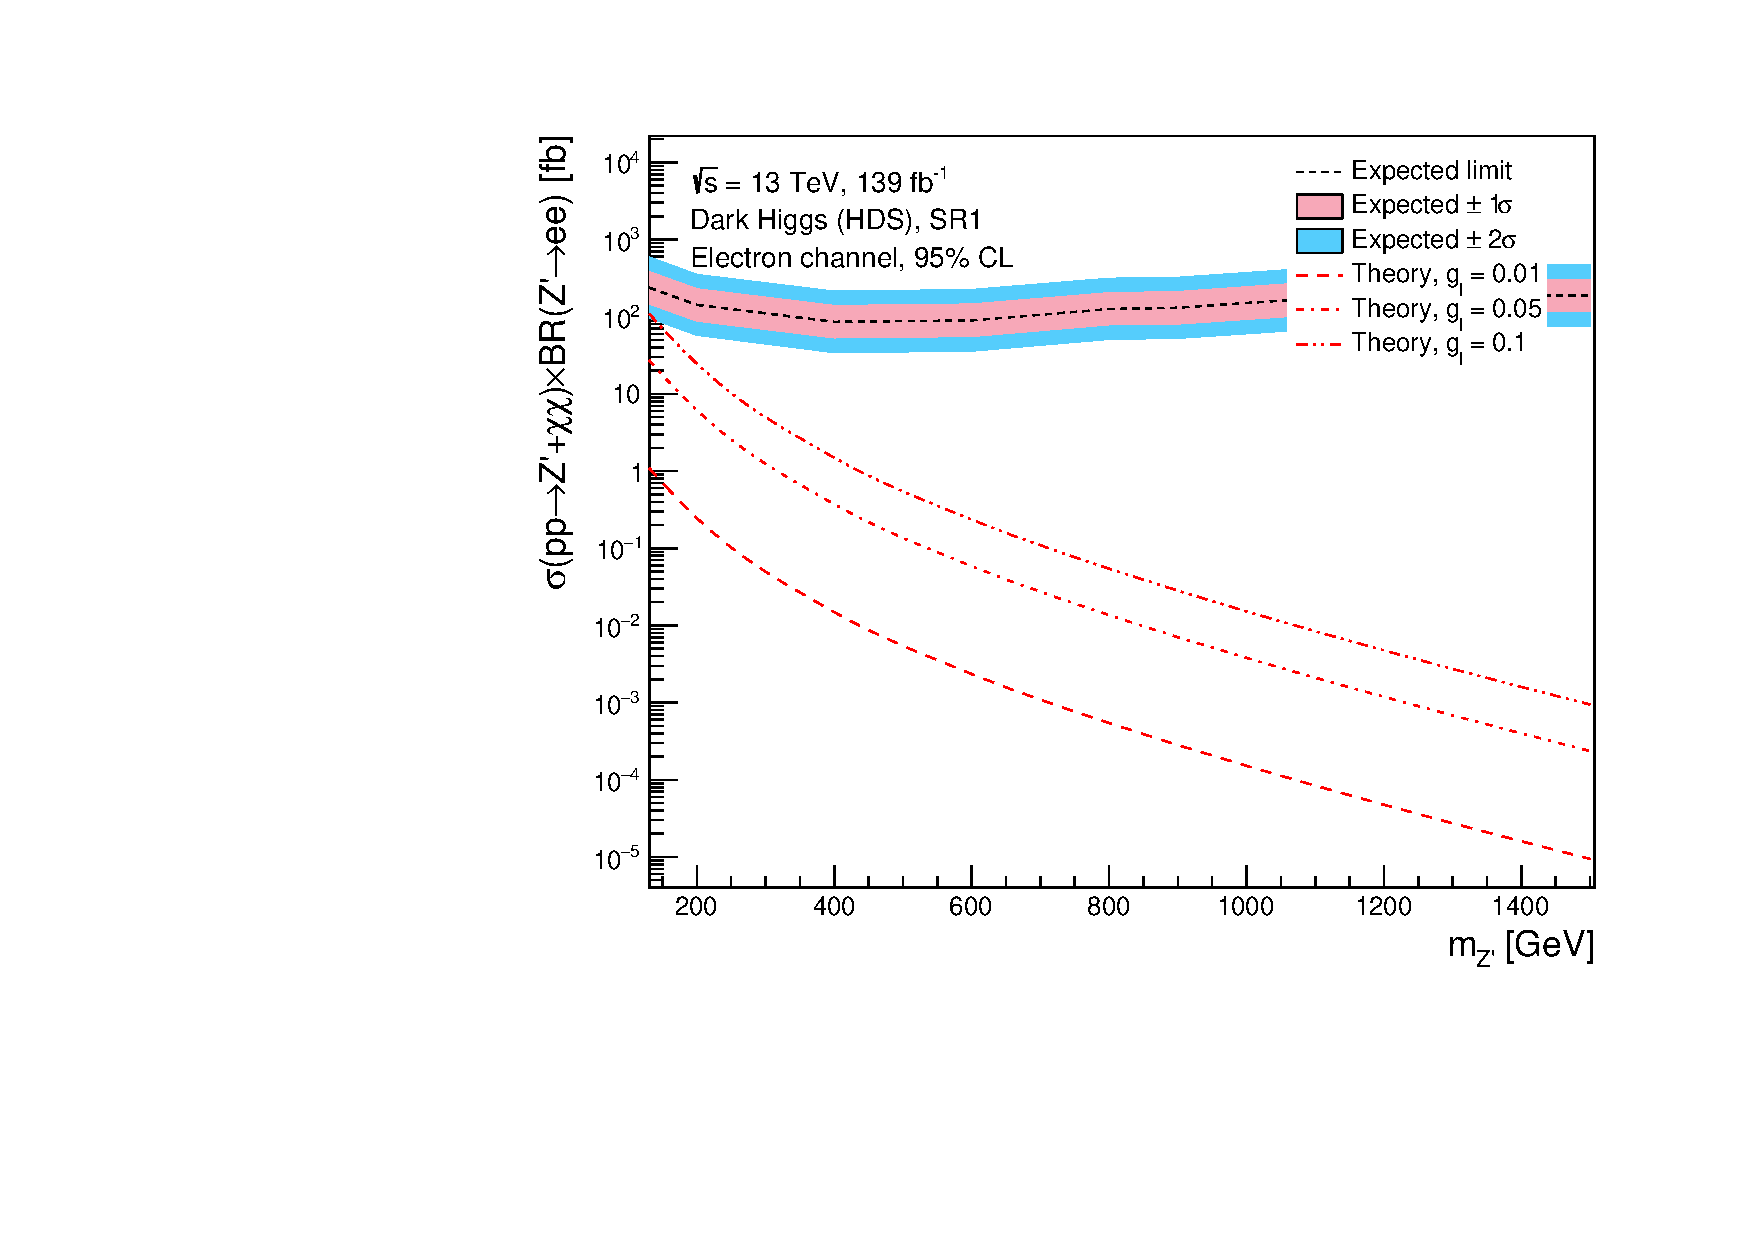
\includegraphics[width=1\textwidth]{Limits/Model_independent/50-100/DH_HDS/mass_exclusion_ee.pdf}
   \end{subfigure}
   \hfill
   \begin{subfigure}[b]{0.49\textwidth}
      \centering
      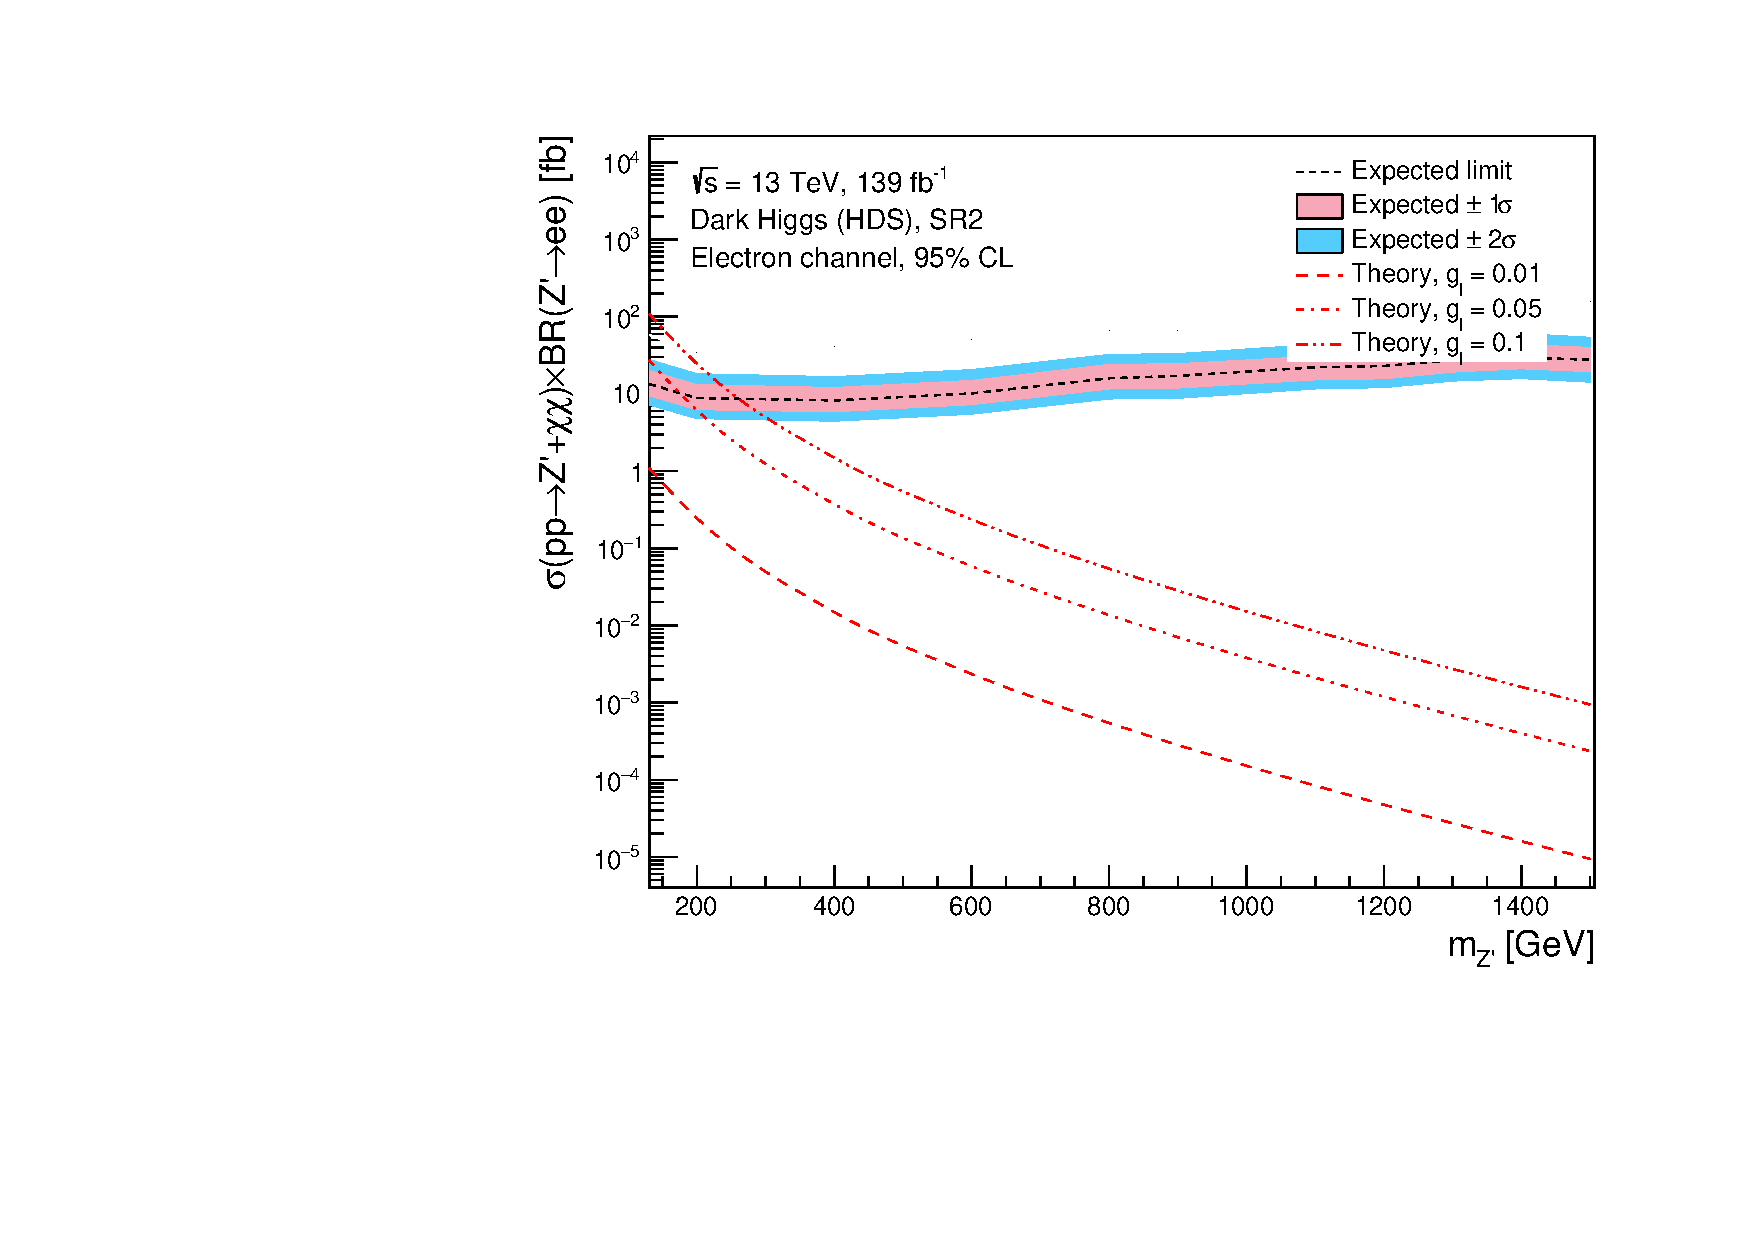
\includegraphics[width=1\textwidth]{Limits/Model_independent/100-150/DH_HDS/mass_exclusion_ee.pdf}
   \end{subfigure}
   \hfill
	\begin{subfigure}[b]{0.49\textwidth}
      \centering
      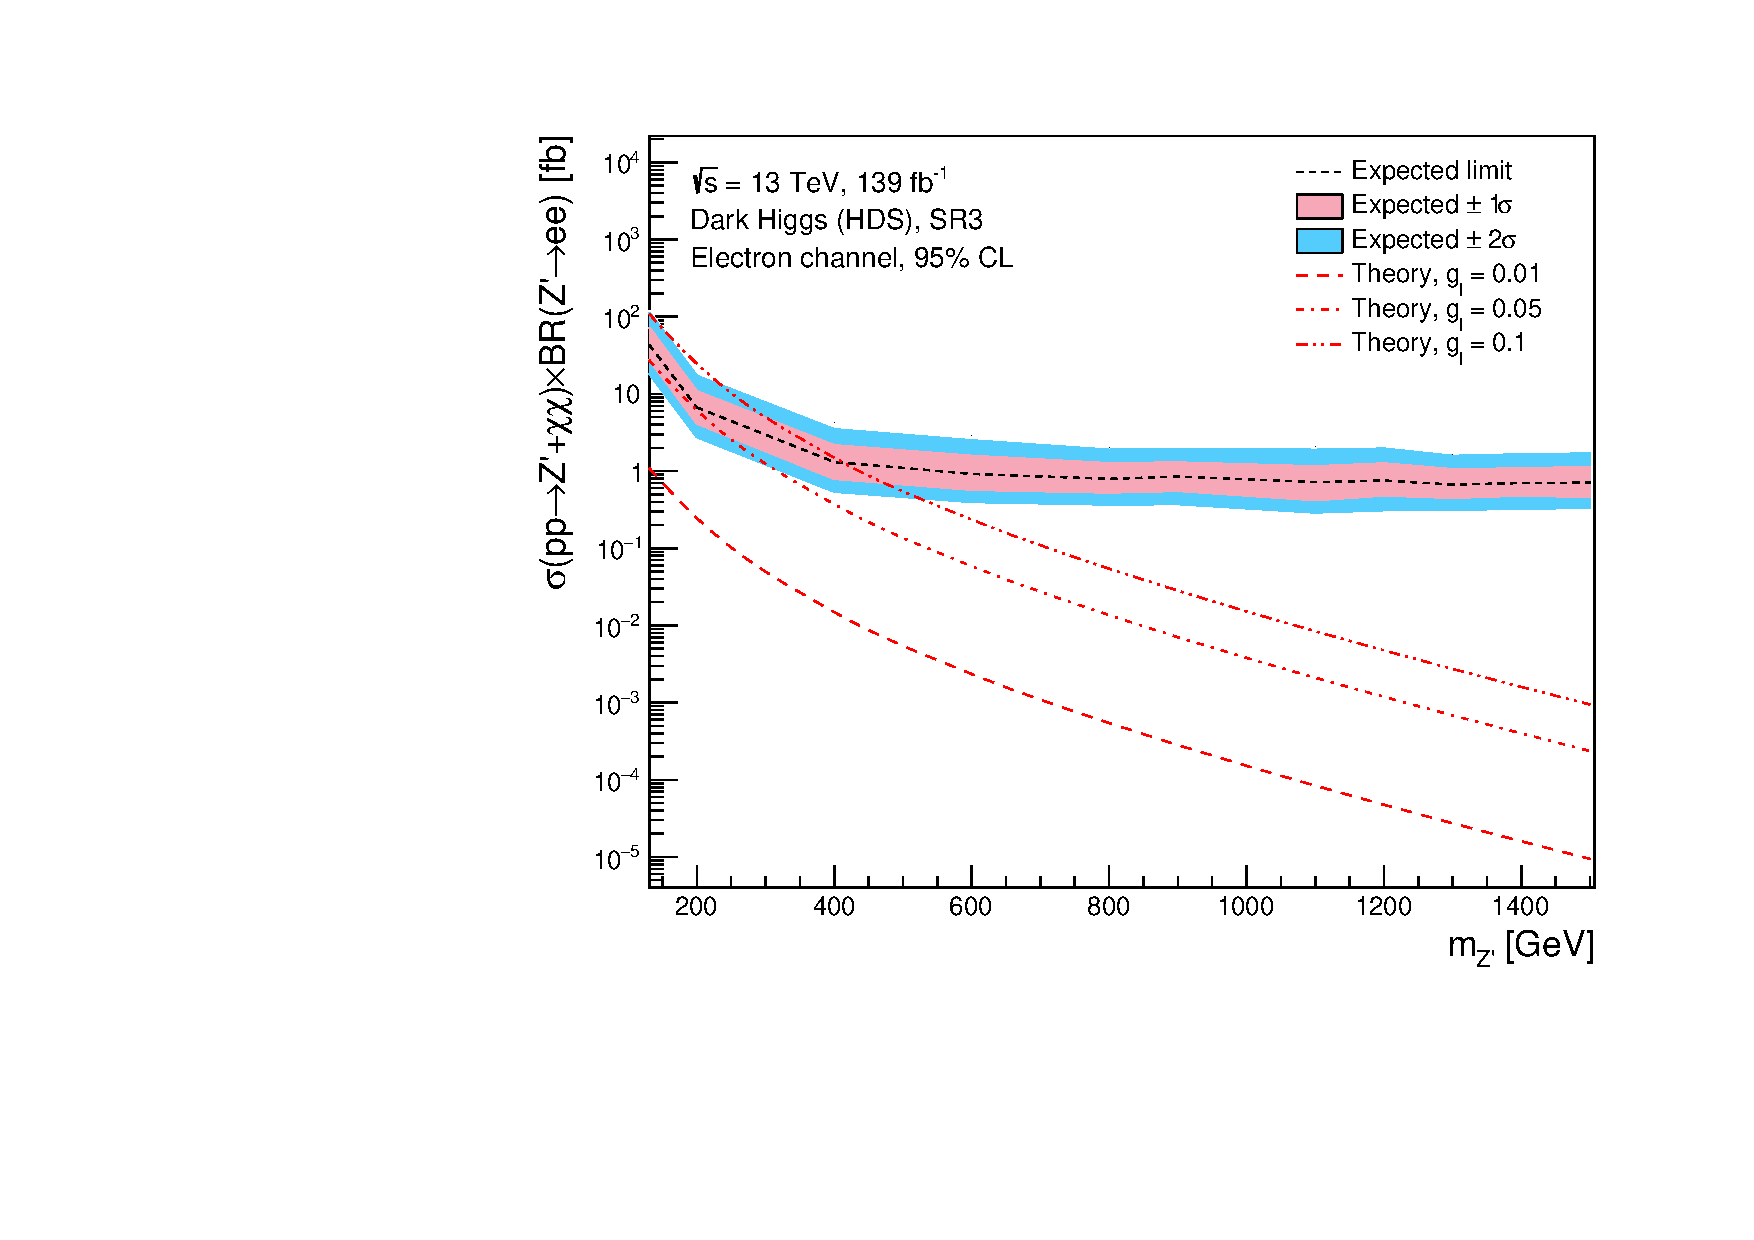
\includegraphics[width=1\textwidth]{Limits/Model_independent/150/DH_HDS/mass_exclusion_ee.pdf}
   \end{subfigure}
   \hfil\begin{subfigure}[b]{0.49\textwidth}
    \centering
    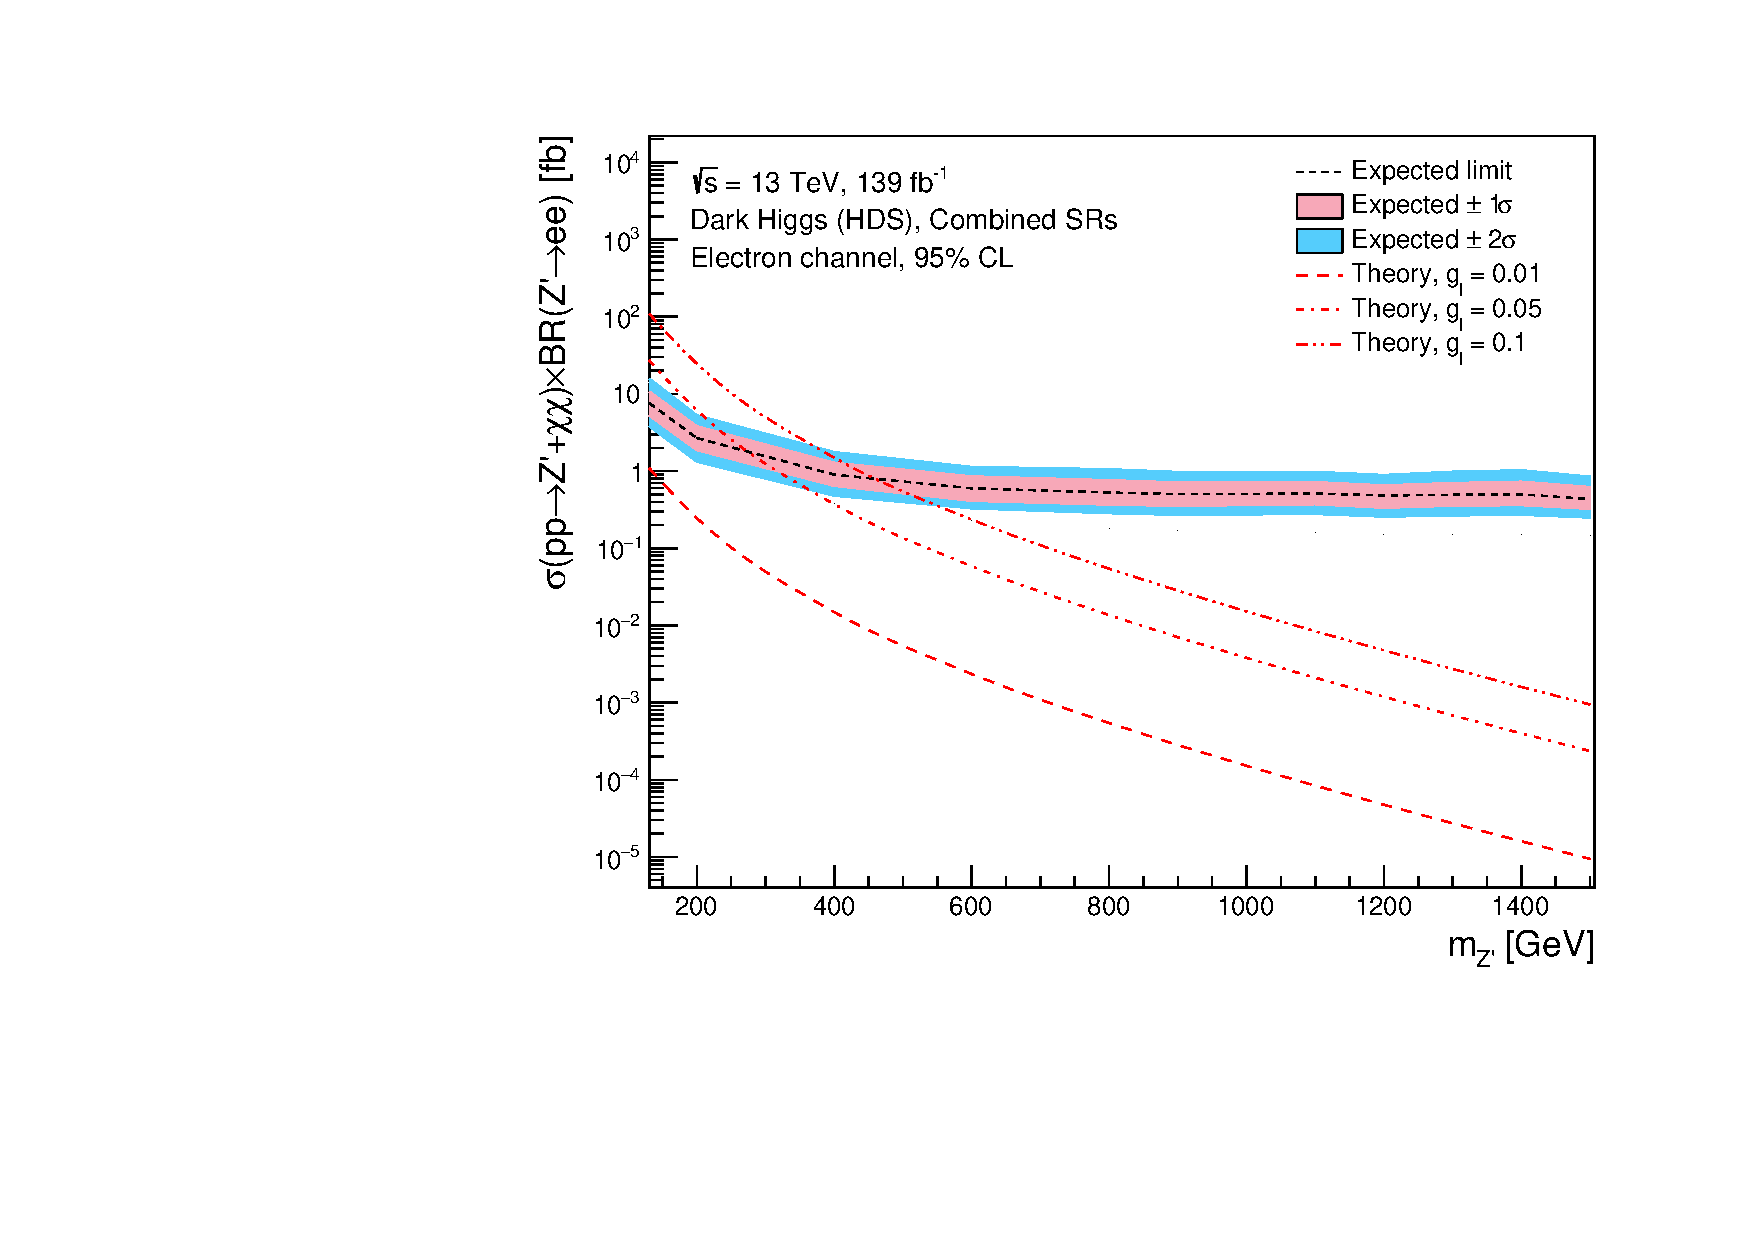
\includegraphics[width=1\textwidth]{Limits/Model_independent/DH_HDS/mass_exclusion_ee.pdf}
 \end{subfigure}
   \caption[Electron channel mass exclusions in DH HDS using the model independent approach]{Mass exclusion limits results for DH HDS model on $ee$ channel in all SRs, including the combined SR channel.}\label{fig:DH_HDS_me_SRS}
\end{figure} 
\\ This can be generalized for every single model we have available, the exclusion limits for the combined dilepton channel and combined SRs for the other models can be seen in Chapter \ref{fig:model_indep_exclusions}. 
To see all the plots used to arrive at these limits for every model you can see the GitHub repo\footnote{Available here: \href{https://github.com/rubenguevara/Master-Thesis/tree/master/Plots/XGBoost}{https://github.com/rubenguevara/Master-Thesis/tree/master/Plots\\/XGBoost}}, 
and to see all the tables with inputs see Appendix \ref{chap:Limit_Tabs}.

\clearpage
\section{Mass exclusion limits for model dependent method}\label{fig:model_dep_exclusions}
\begin{figure}[!ht]
	\centering
	\begin{subfigure}[b]{0.49\textwidth}
      \centering
      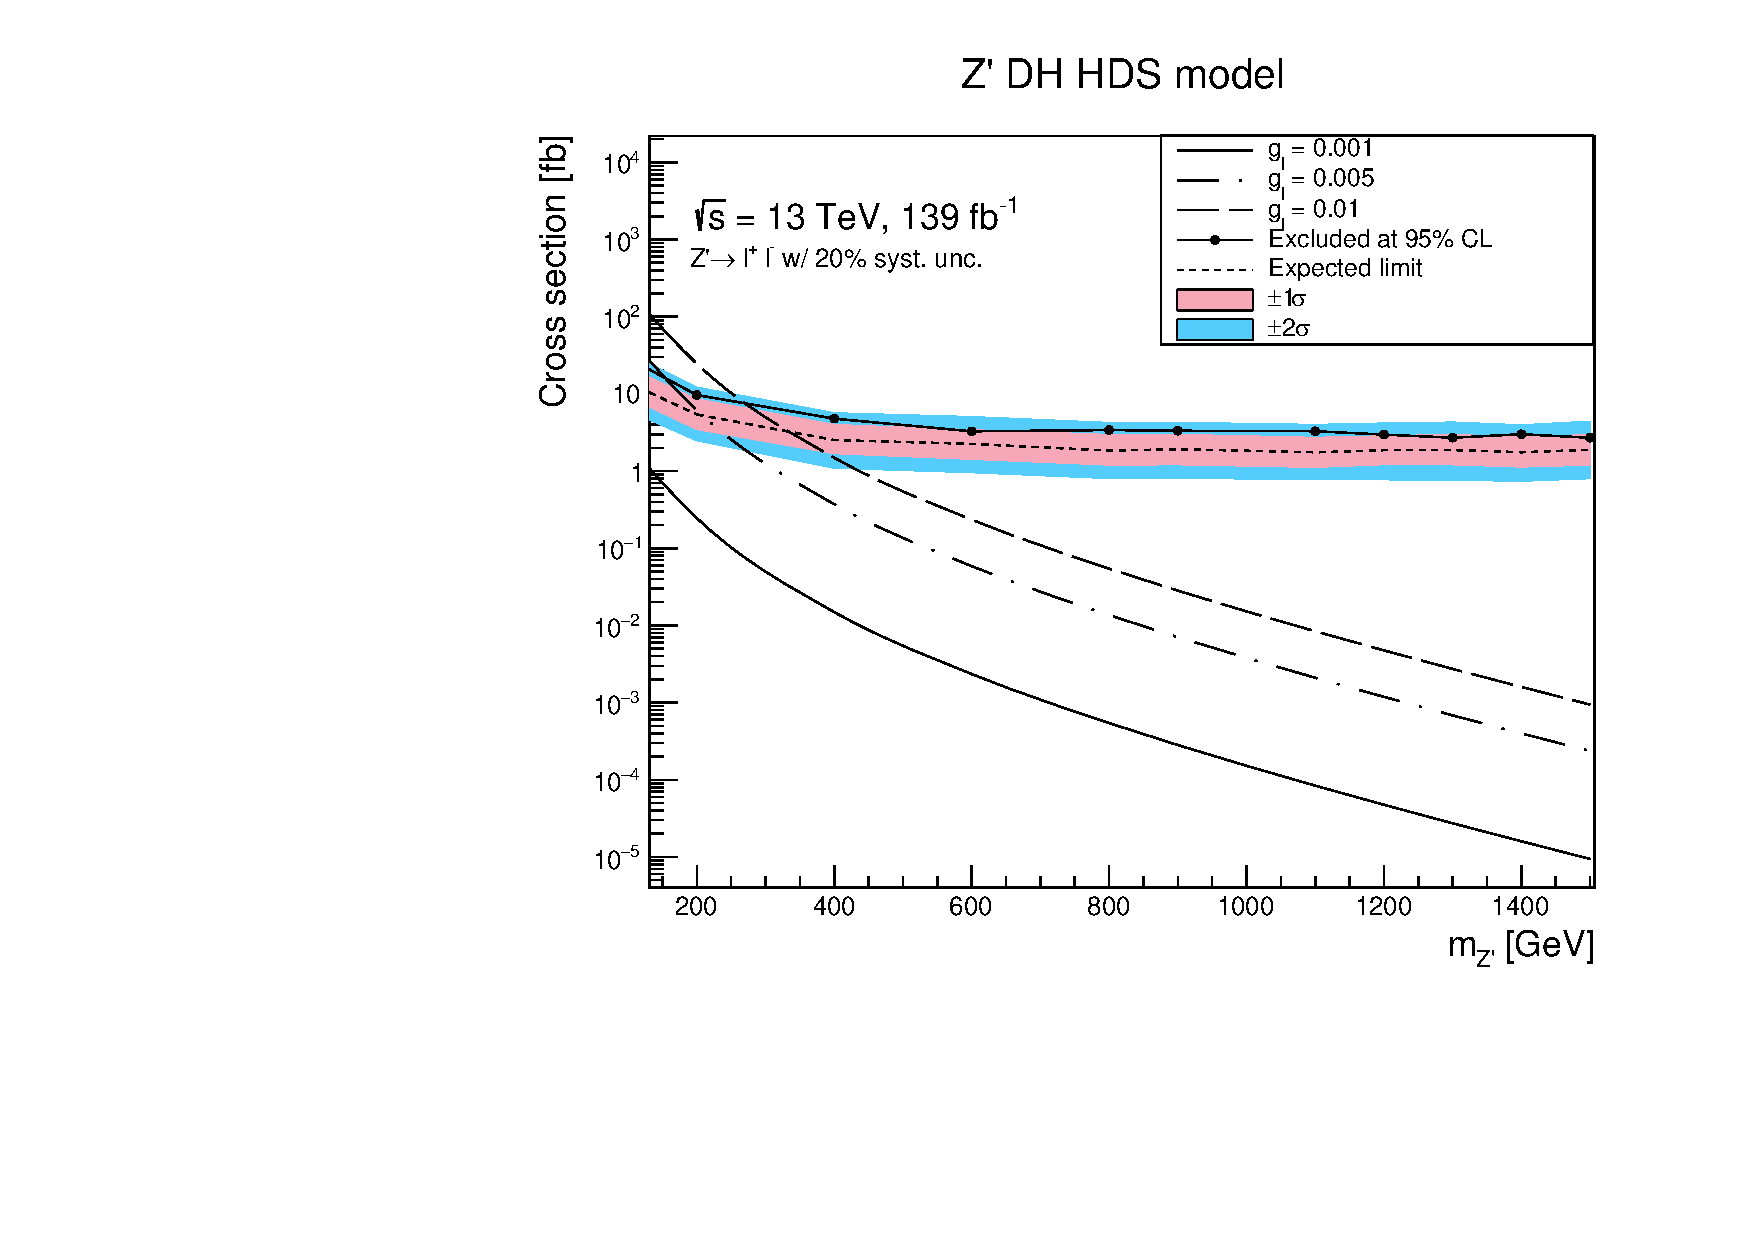
\includegraphics[width=1\textwidth]{Limits/DH_HDS/mass_exclusion_comb.pdf}
   \end{subfigure}
   \hfill
   \begin{subfigure}[b]{0.49\textwidth}
      \centering
      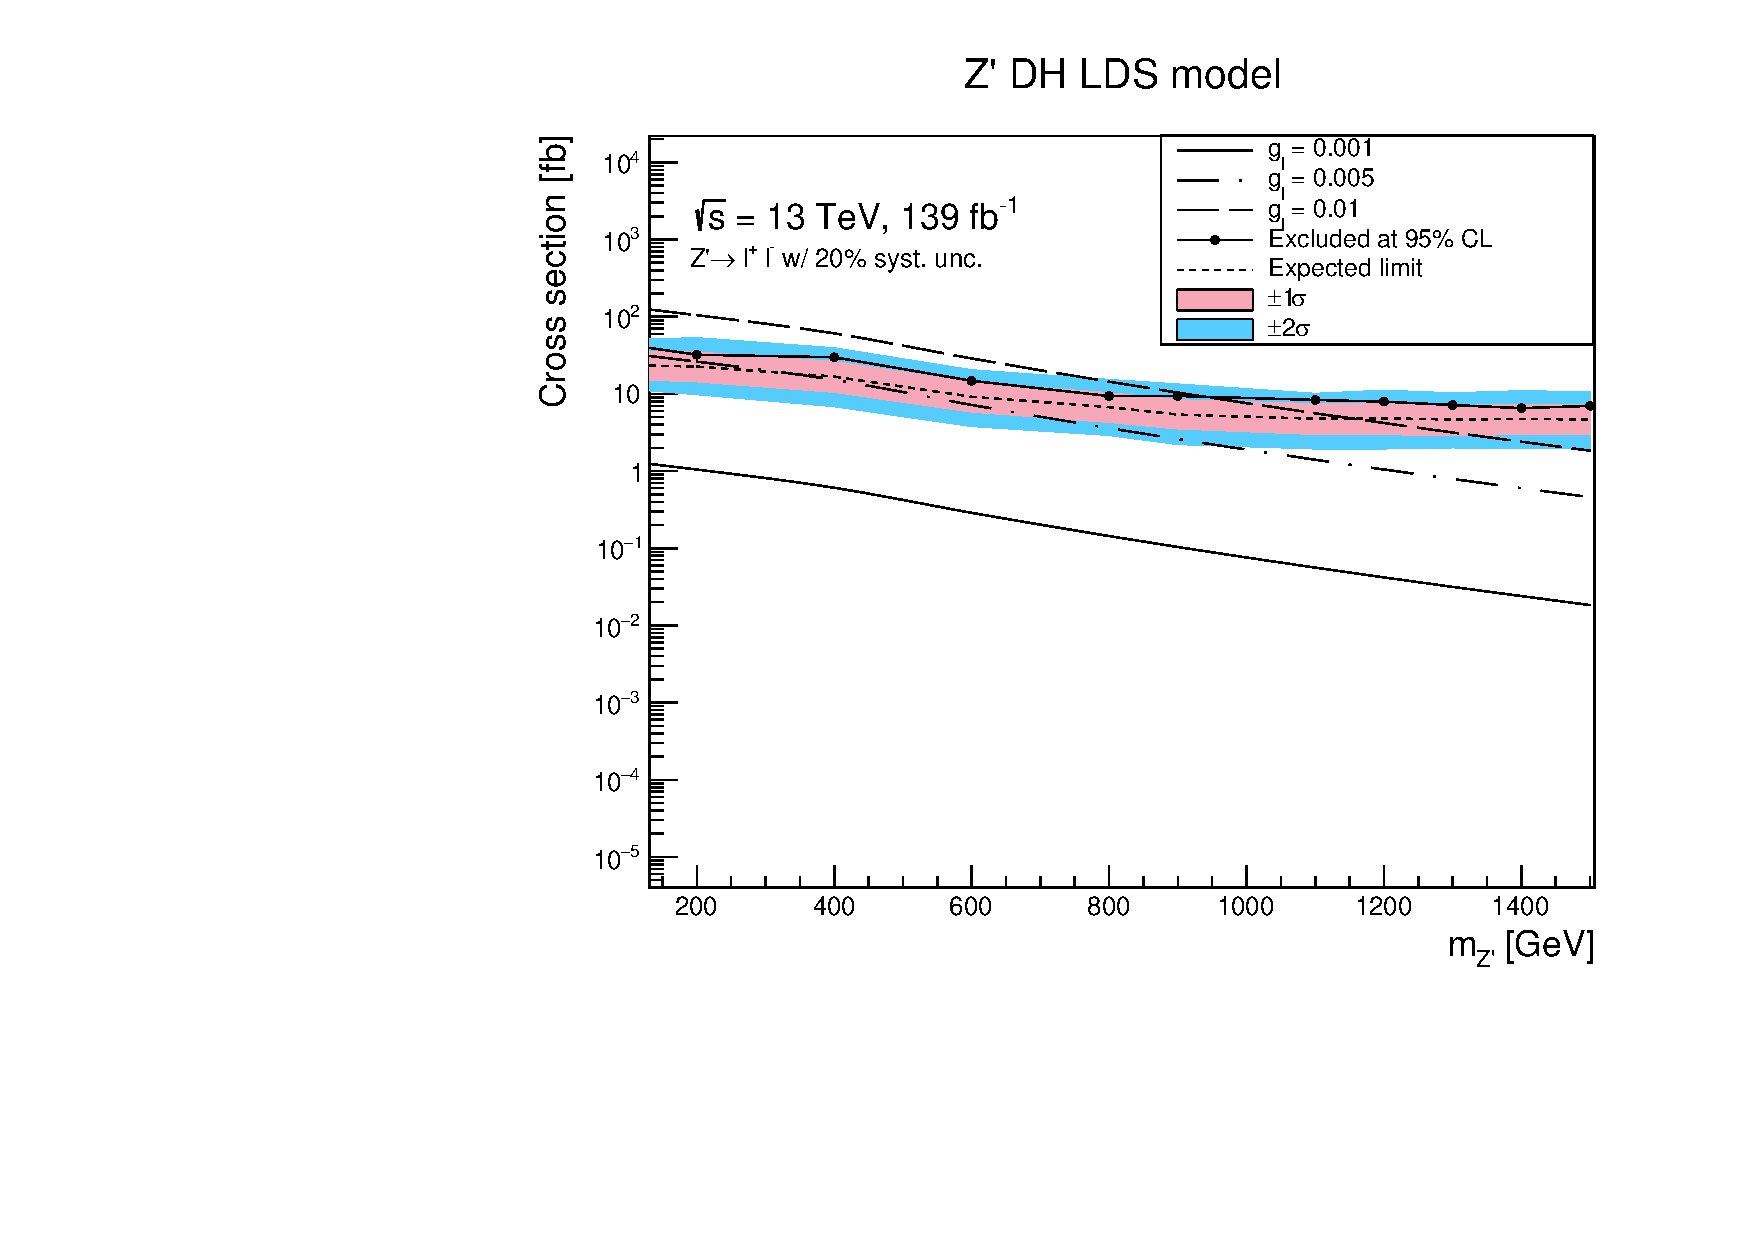
\includegraphics[width=1\textwidth]{Limits/DH_LDS/mass_exclusion_comb.pdf}
   \end{subfigure}
   \hfill
   \begin{subfigure}[b]{0.49\textwidth}
      \centering
      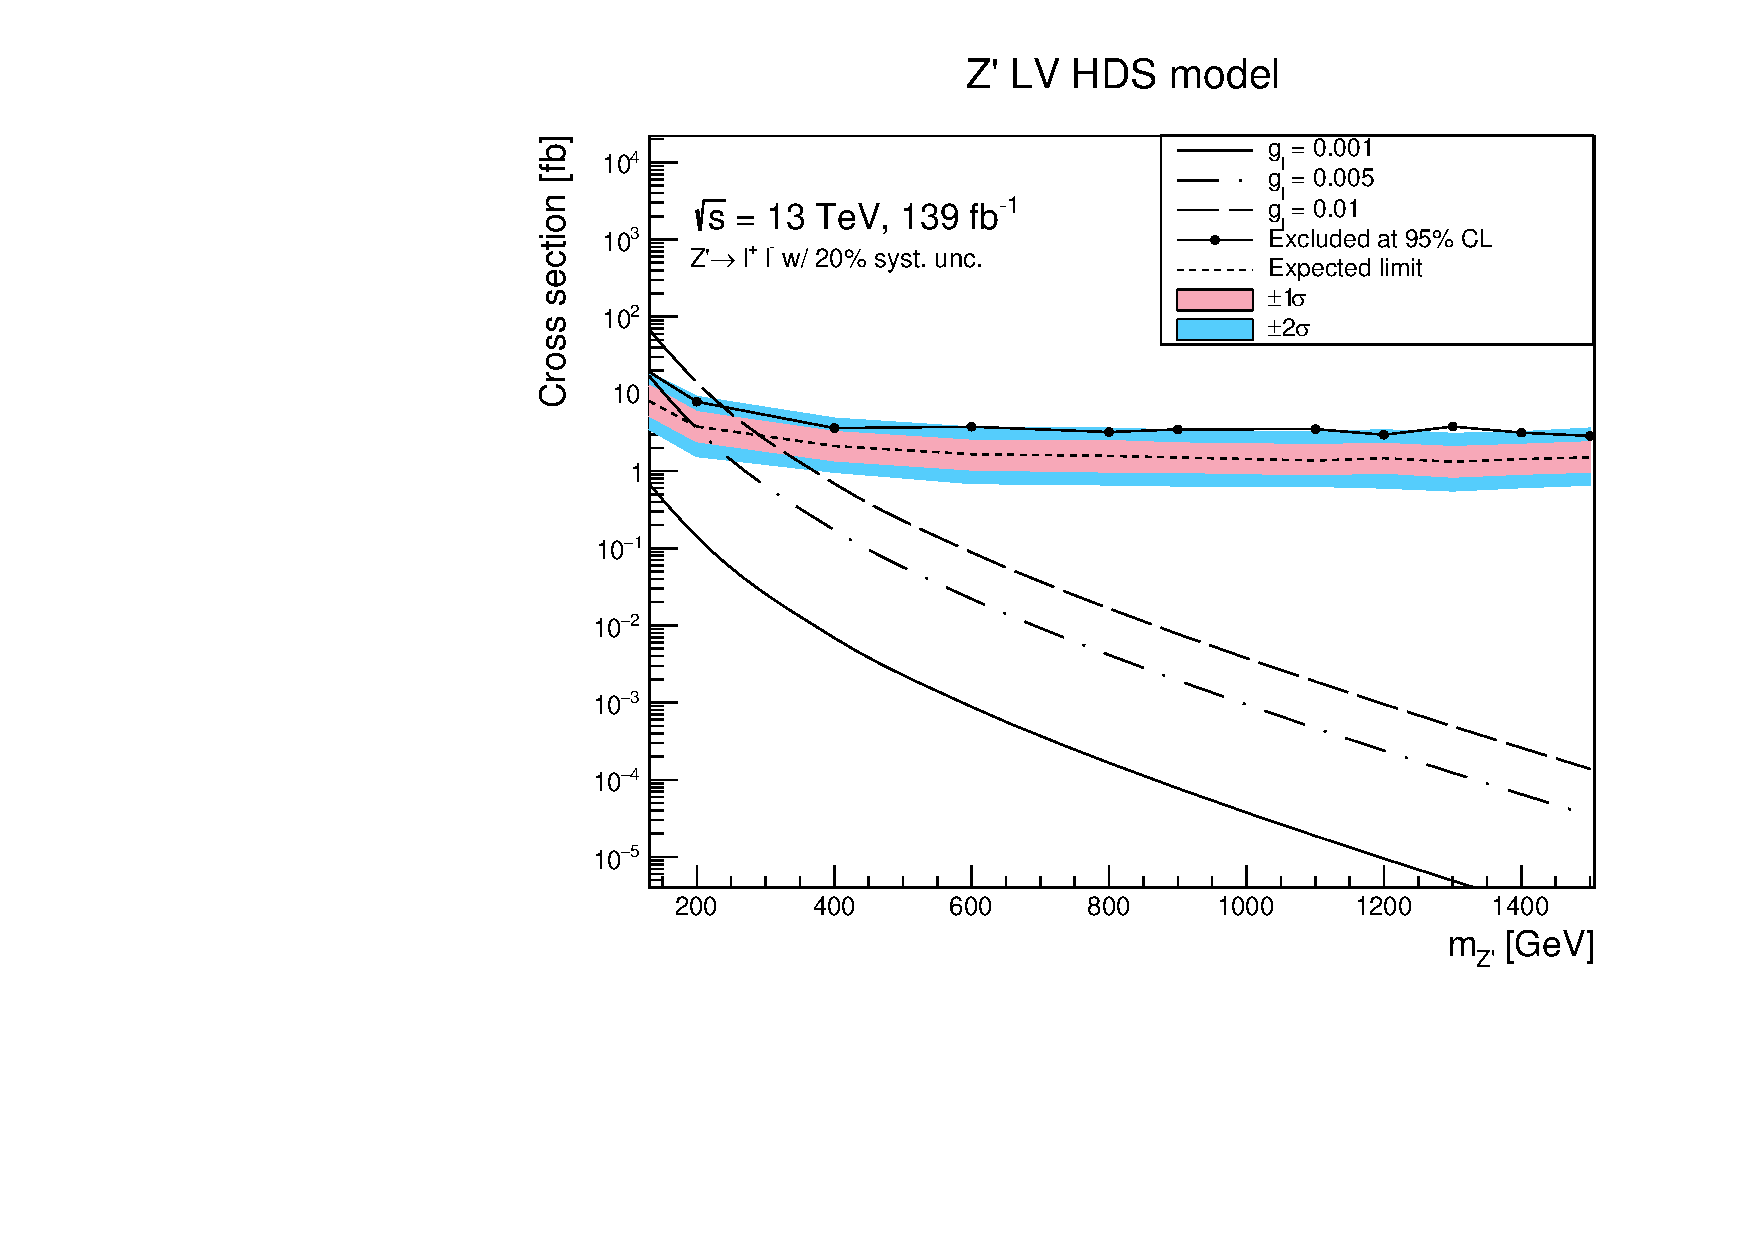
\includegraphics[width=1\textwidth]{Limits/LV_HDS/mass_exclusion_comb.pdf}
   \end{subfigure}
   \hfill
   \begin{subfigure}[b]{0.49\textwidth}
      \centering
      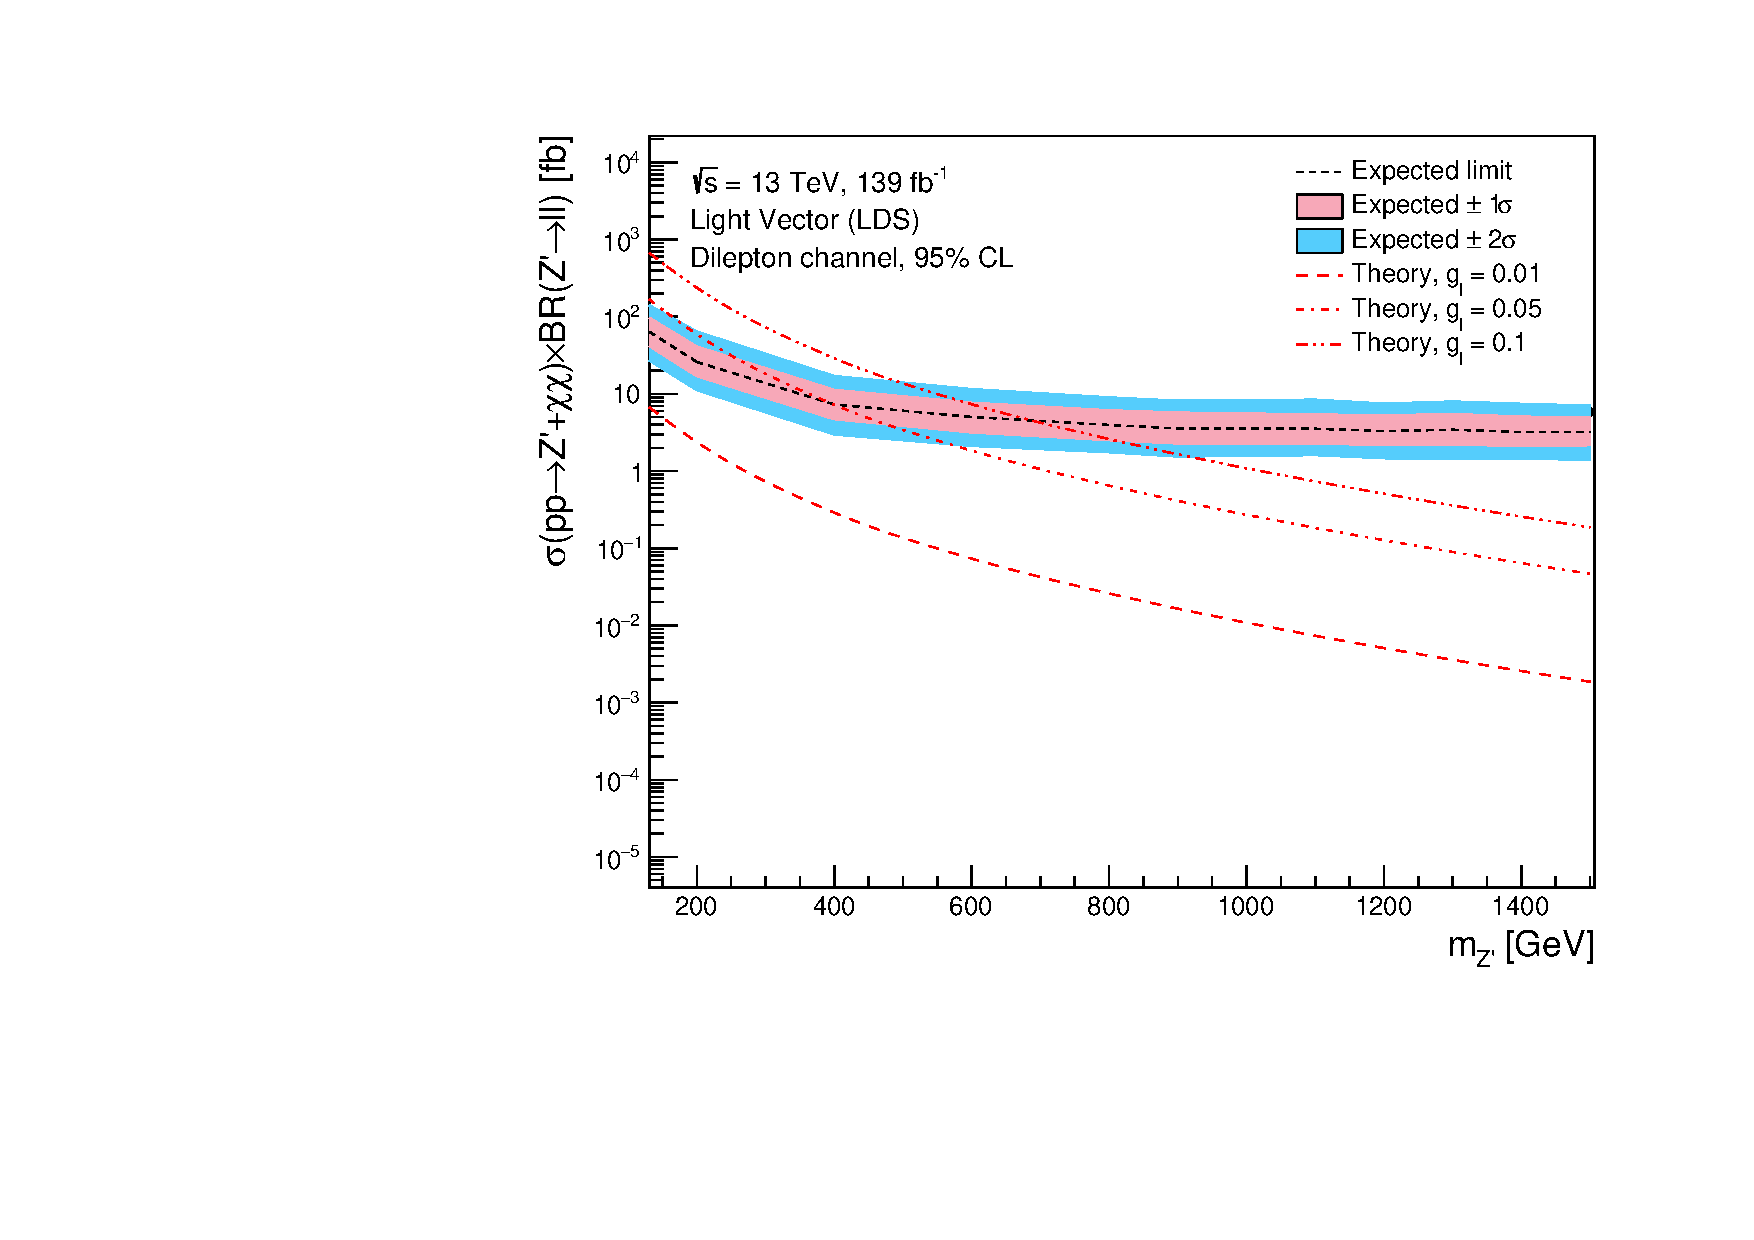
\includegraphics[width=1\textwidth]{Limits/LV_LDS/mass_exclusion_comb.pdf}
   \end{subfigure}
   \hfill
	\begin{subfigure}[b]{0.49\textwidth}
      \centering
      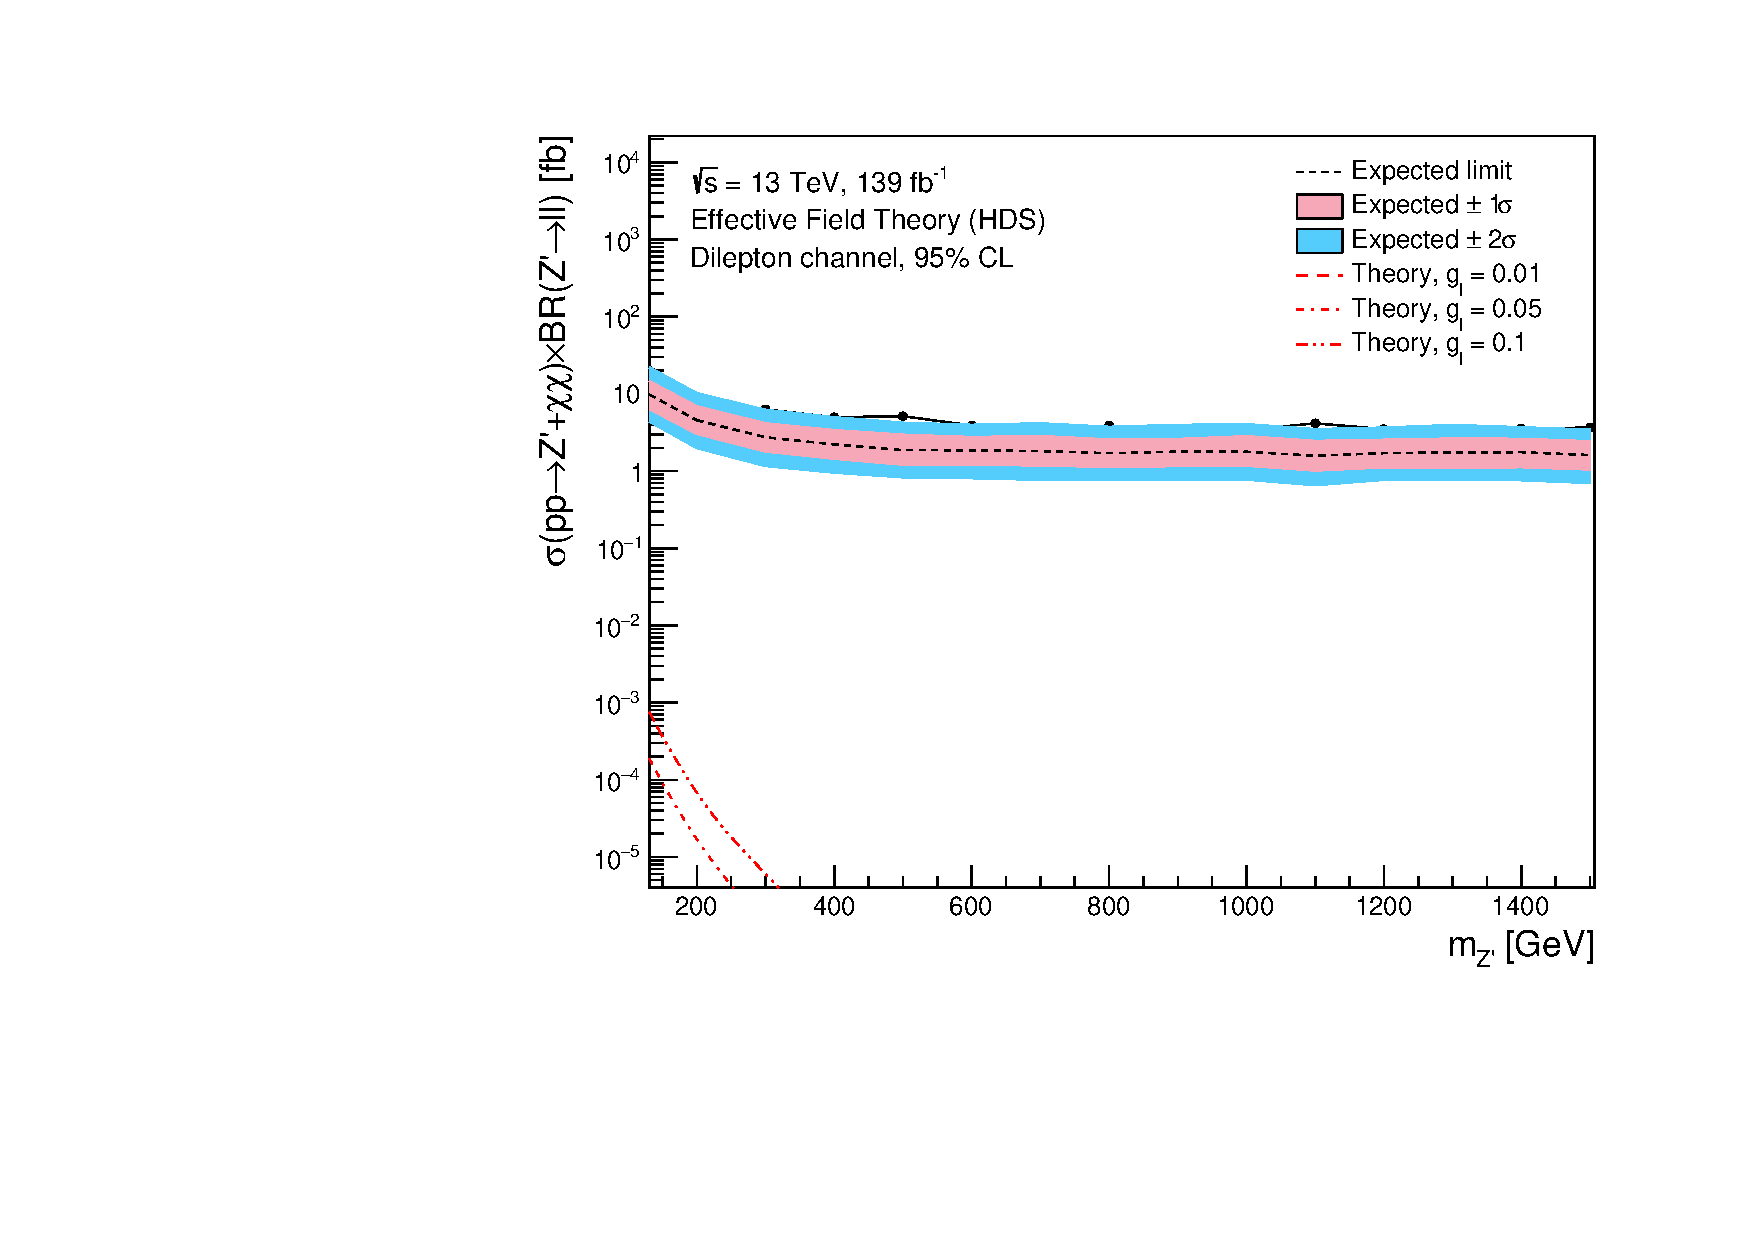
\includegraphics[width=1\textwidth]{Limits/EFT_HDS/mass_exclusion_comb.pdf}
   \end{subfigure}
   \hfill
   \begin{subfigure}[b]{0.49\textwidth}
      \centering
      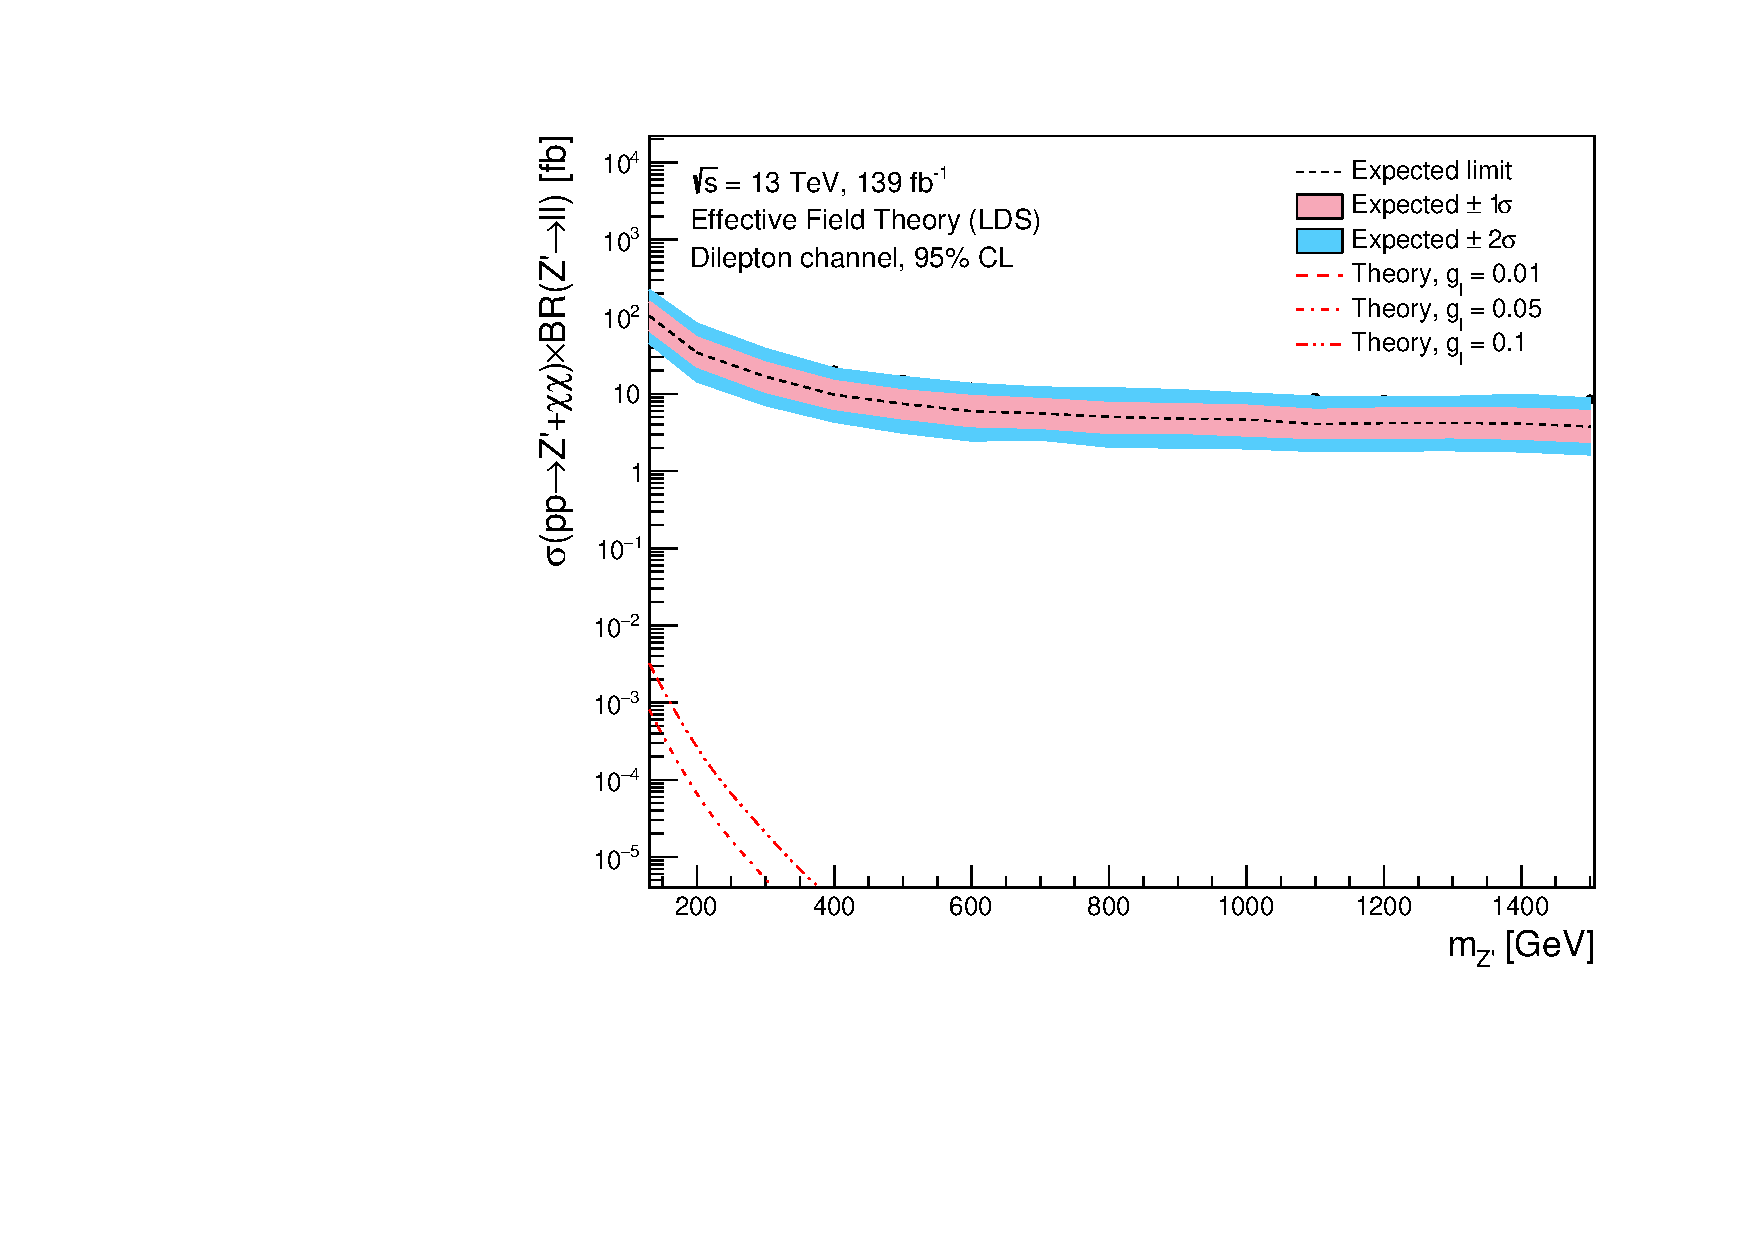
\includegraphics[width=1\textwidth]{Limits/EFT_LDS/mass_exclusion_comb.pdf}
   \end{subfigure}
   \caption[Mass exclusion limits of combined $ee$ and $\mu\mu$ channel for all mono-Z' models using model dependent method]{Mass exclusion limits of combined $ee$ and $\mu\mu$ channel for all mono-Z' models using model dependent method}
\end{figure}
\clearpage


\clearpage
\section{Mass exclusion limits for model independent method}\label{fig:model_indep_exclusions}
\textbf{NB: these will most likely change with the inclusion of the new models!}
\begin{figure}[!ht]
	\centering
	\begin{subfigure}[b]{0.49\textwidth}
      \centering
      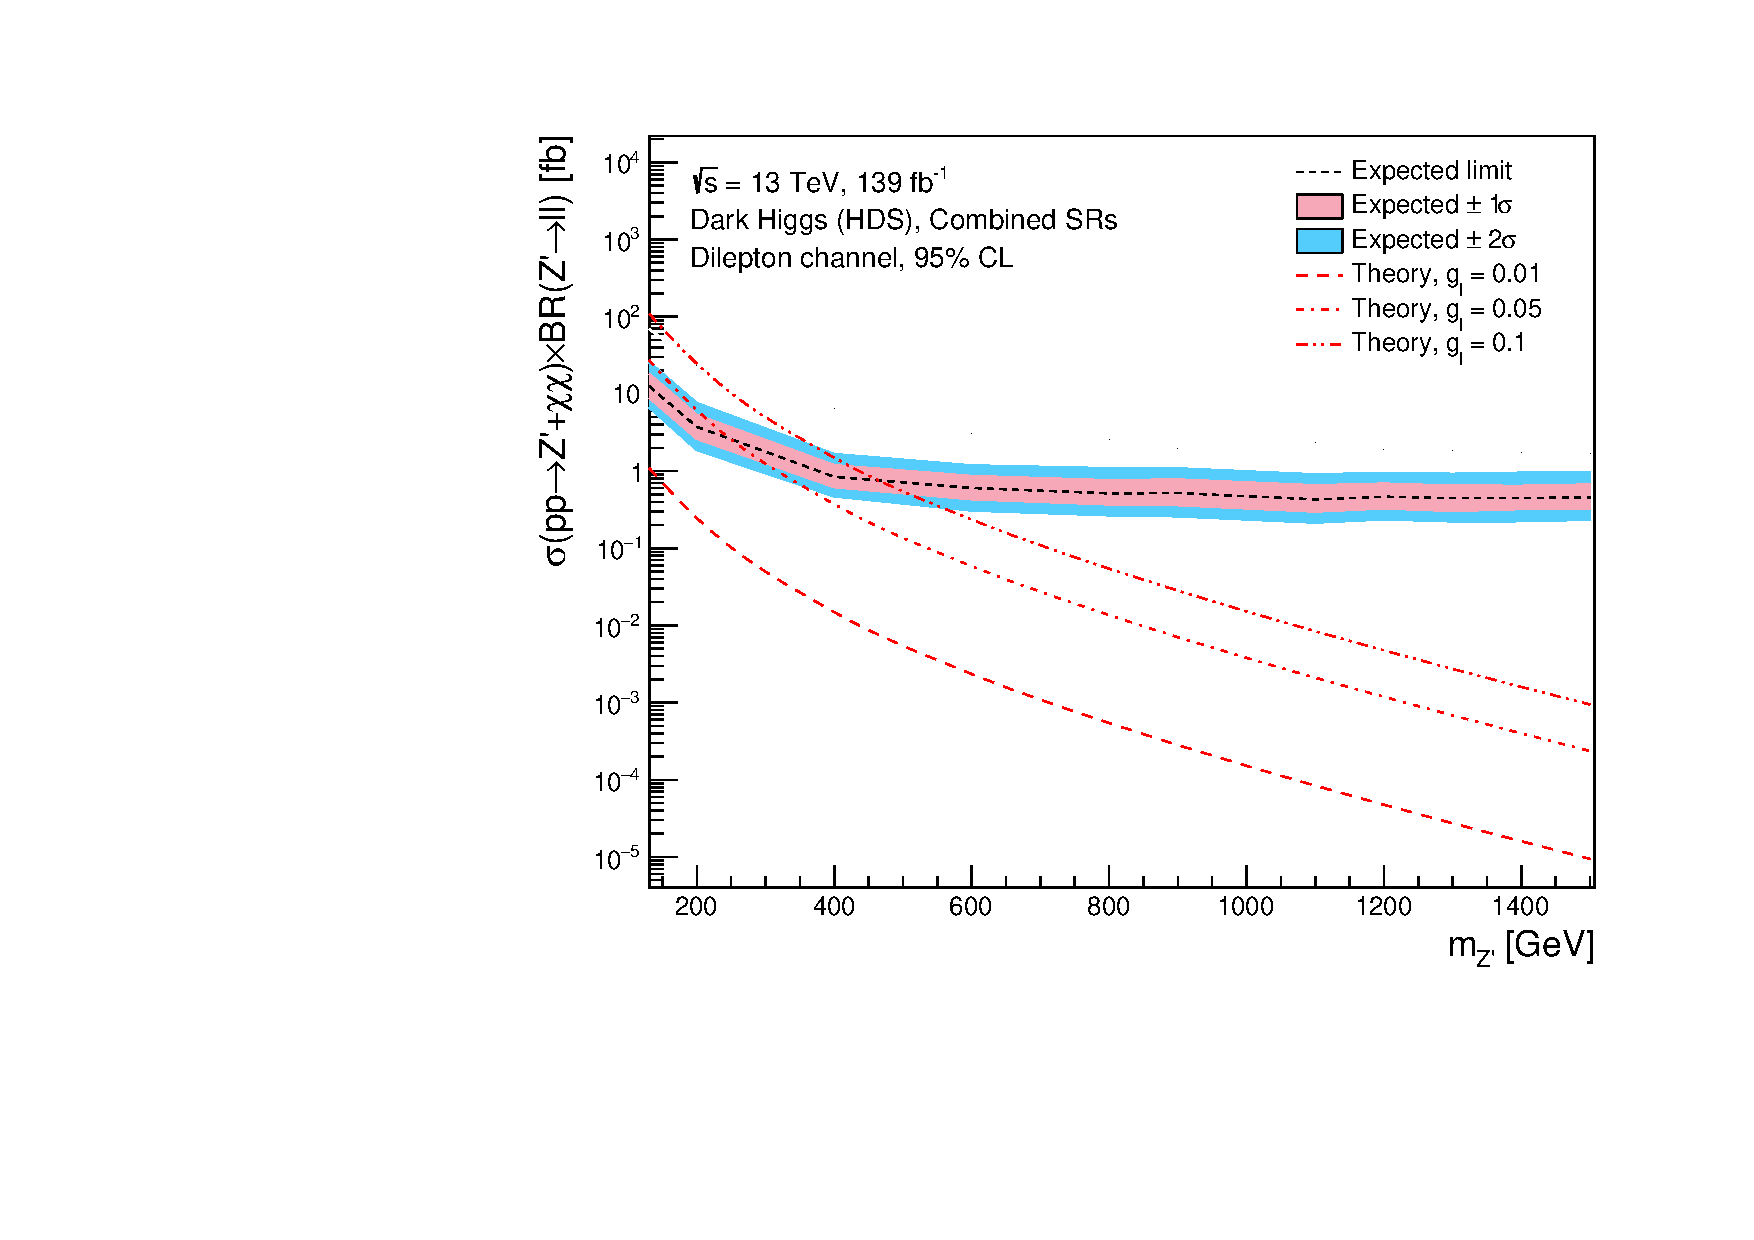
\includegraphics[width=1\textwidth]{Limits/Model_independent/DH_HDS/mass_exclusion_comb.pdf}
   \end{subfigure}
   \hfill
   \begin{subfigure}[b]{0.49\textwidth}
      \centering
      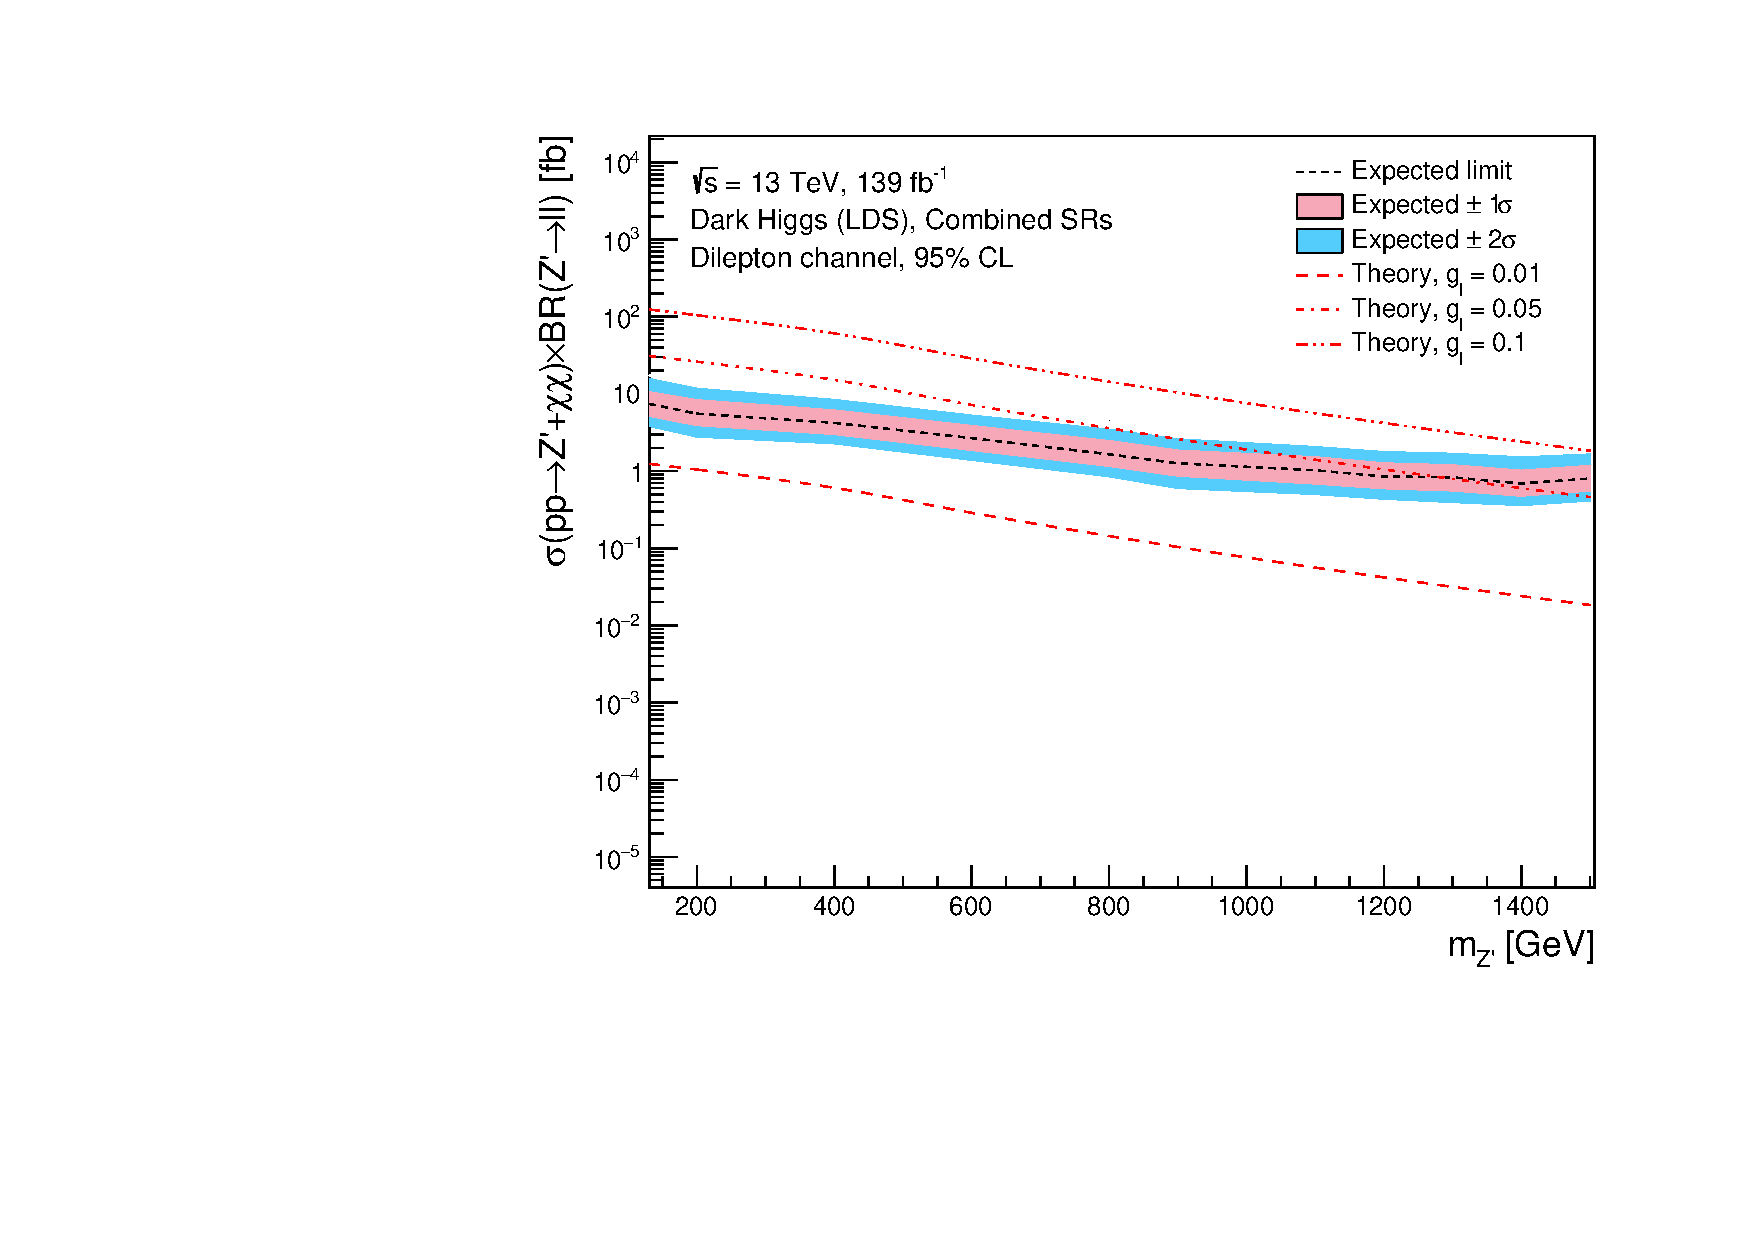
\includegraphics[width=1\textwidth]{Limits/Model_independent/DH_LDS/mass_exclusion_comb.pdf}
   \end{subfigure}
   \hfill
   \begin{subfigure}[b]{0.49\textwidth}
      \centering
      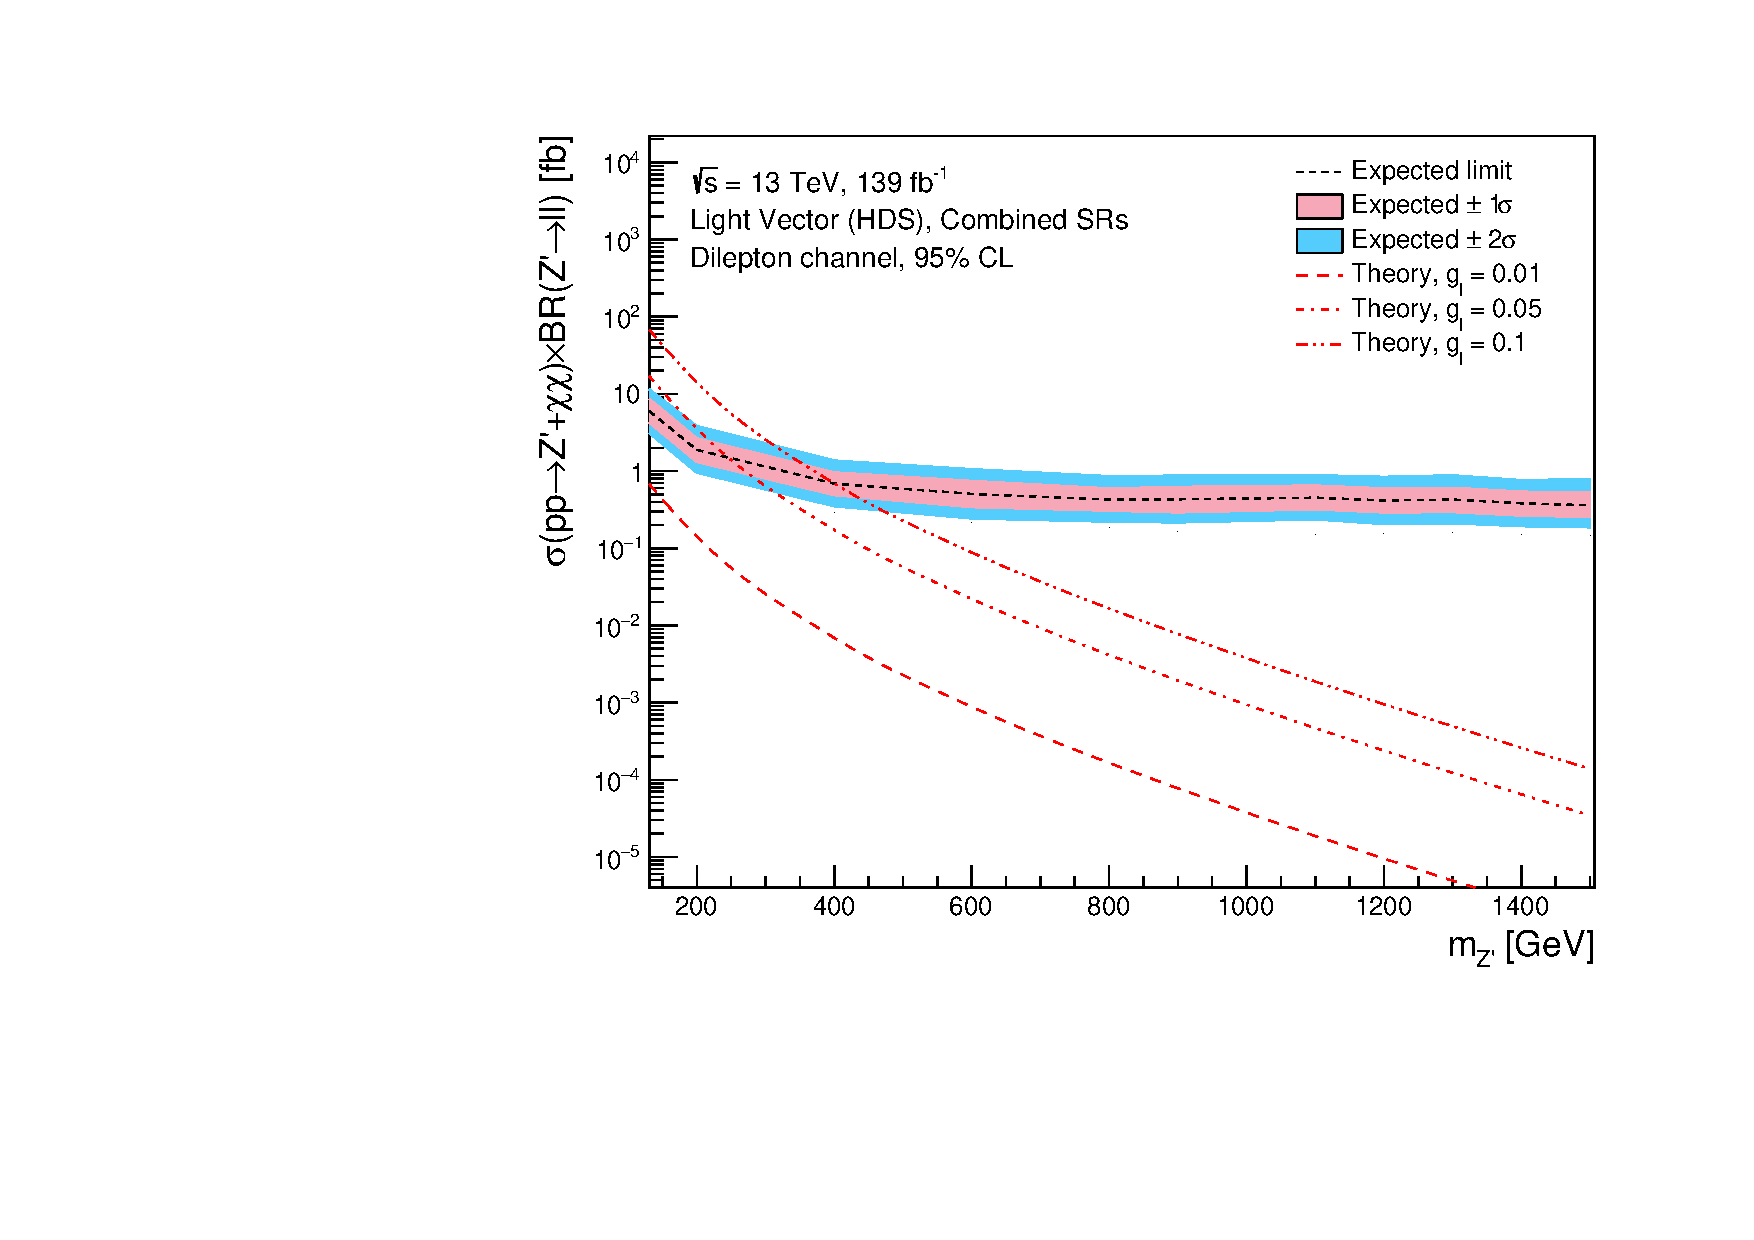
\includegraphics[width=1\textwidth]{Limits/Model_independent/LV_HDS/mass_exclusion_comb.pdf}
   \end{subfigure}
   \hfill
   \begin{subfigure}[b]{0.49\textwidth}
      \centering
      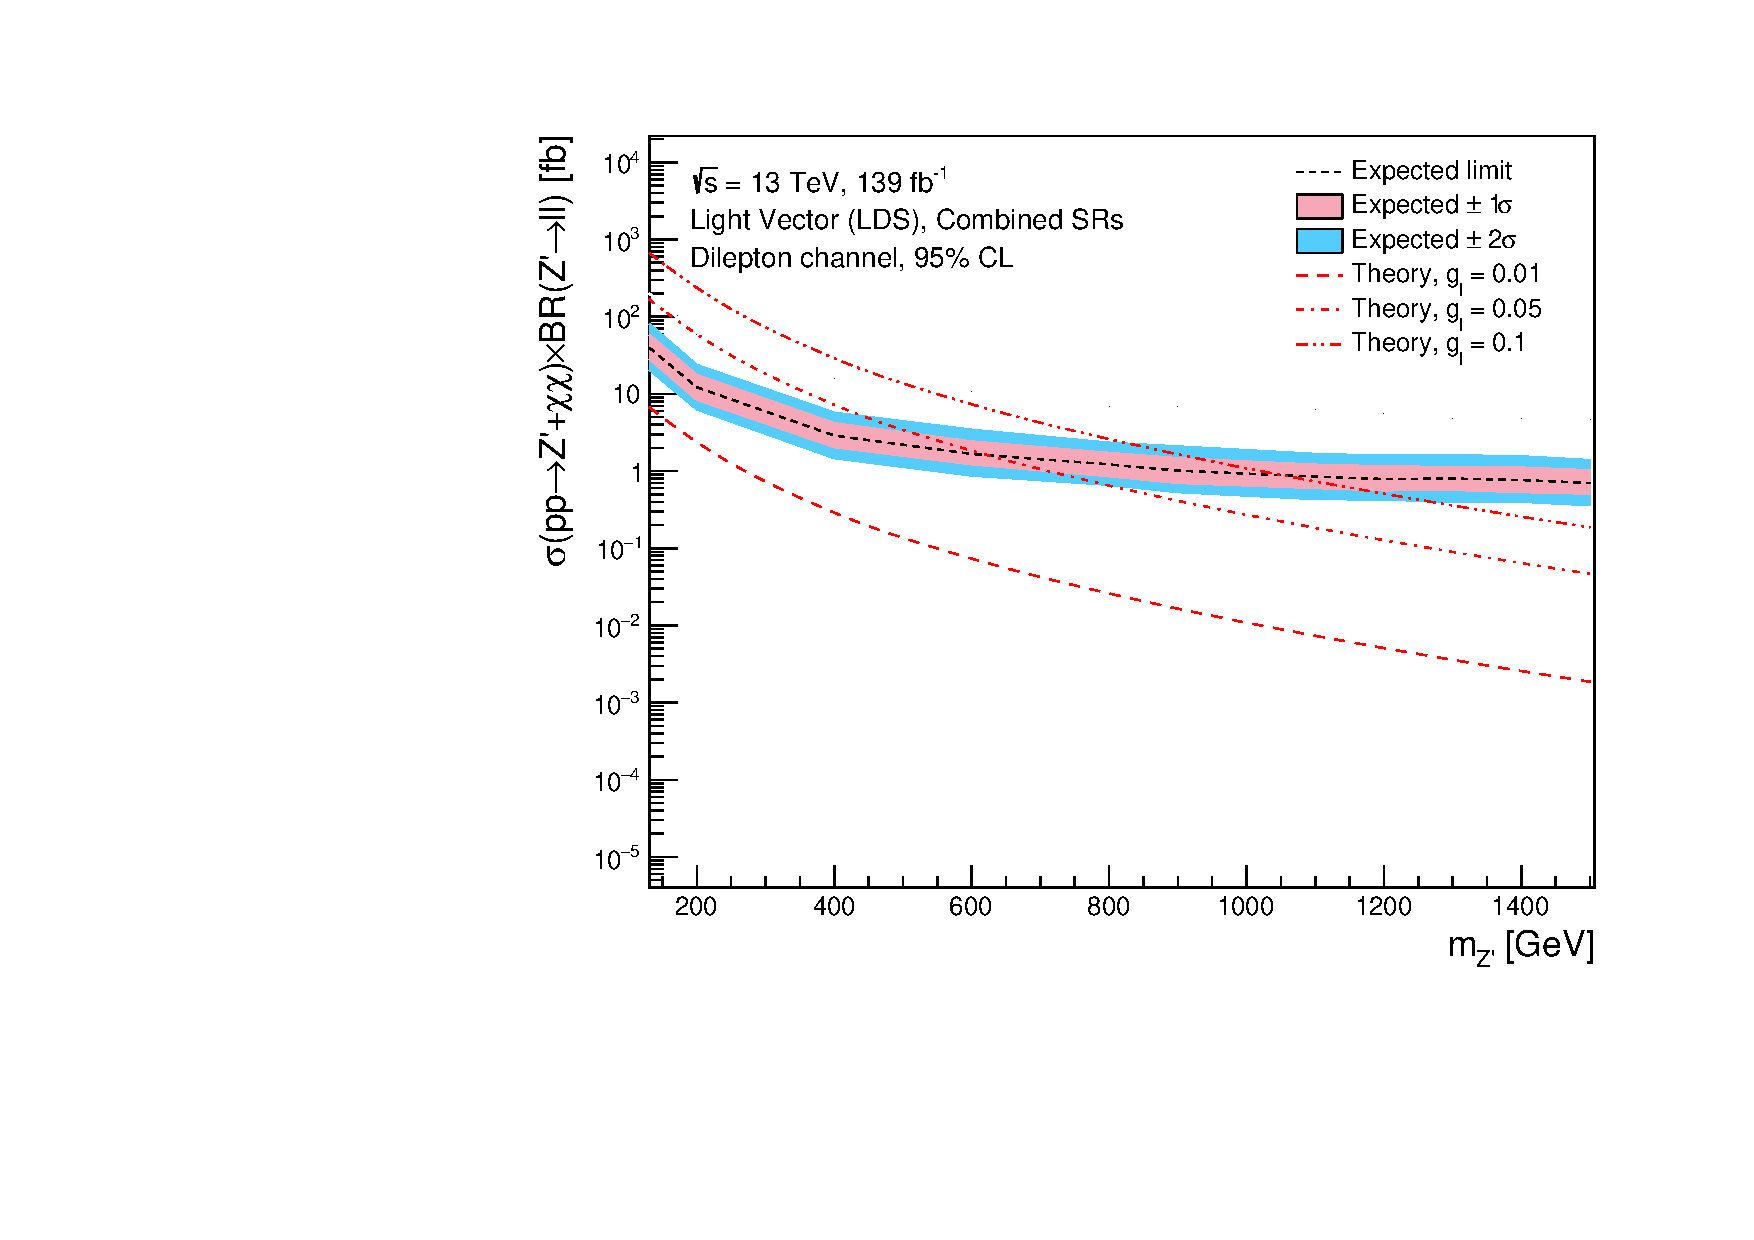
\includegraphics[width=1\textwidth]{Limits/Model_independent/LV_LDS/mass_exclusion_comb.pdf}
   \end{subfigure}
   \hfill
	\begin{subfigure}[b]{0.49\textwidth}
      \centering
      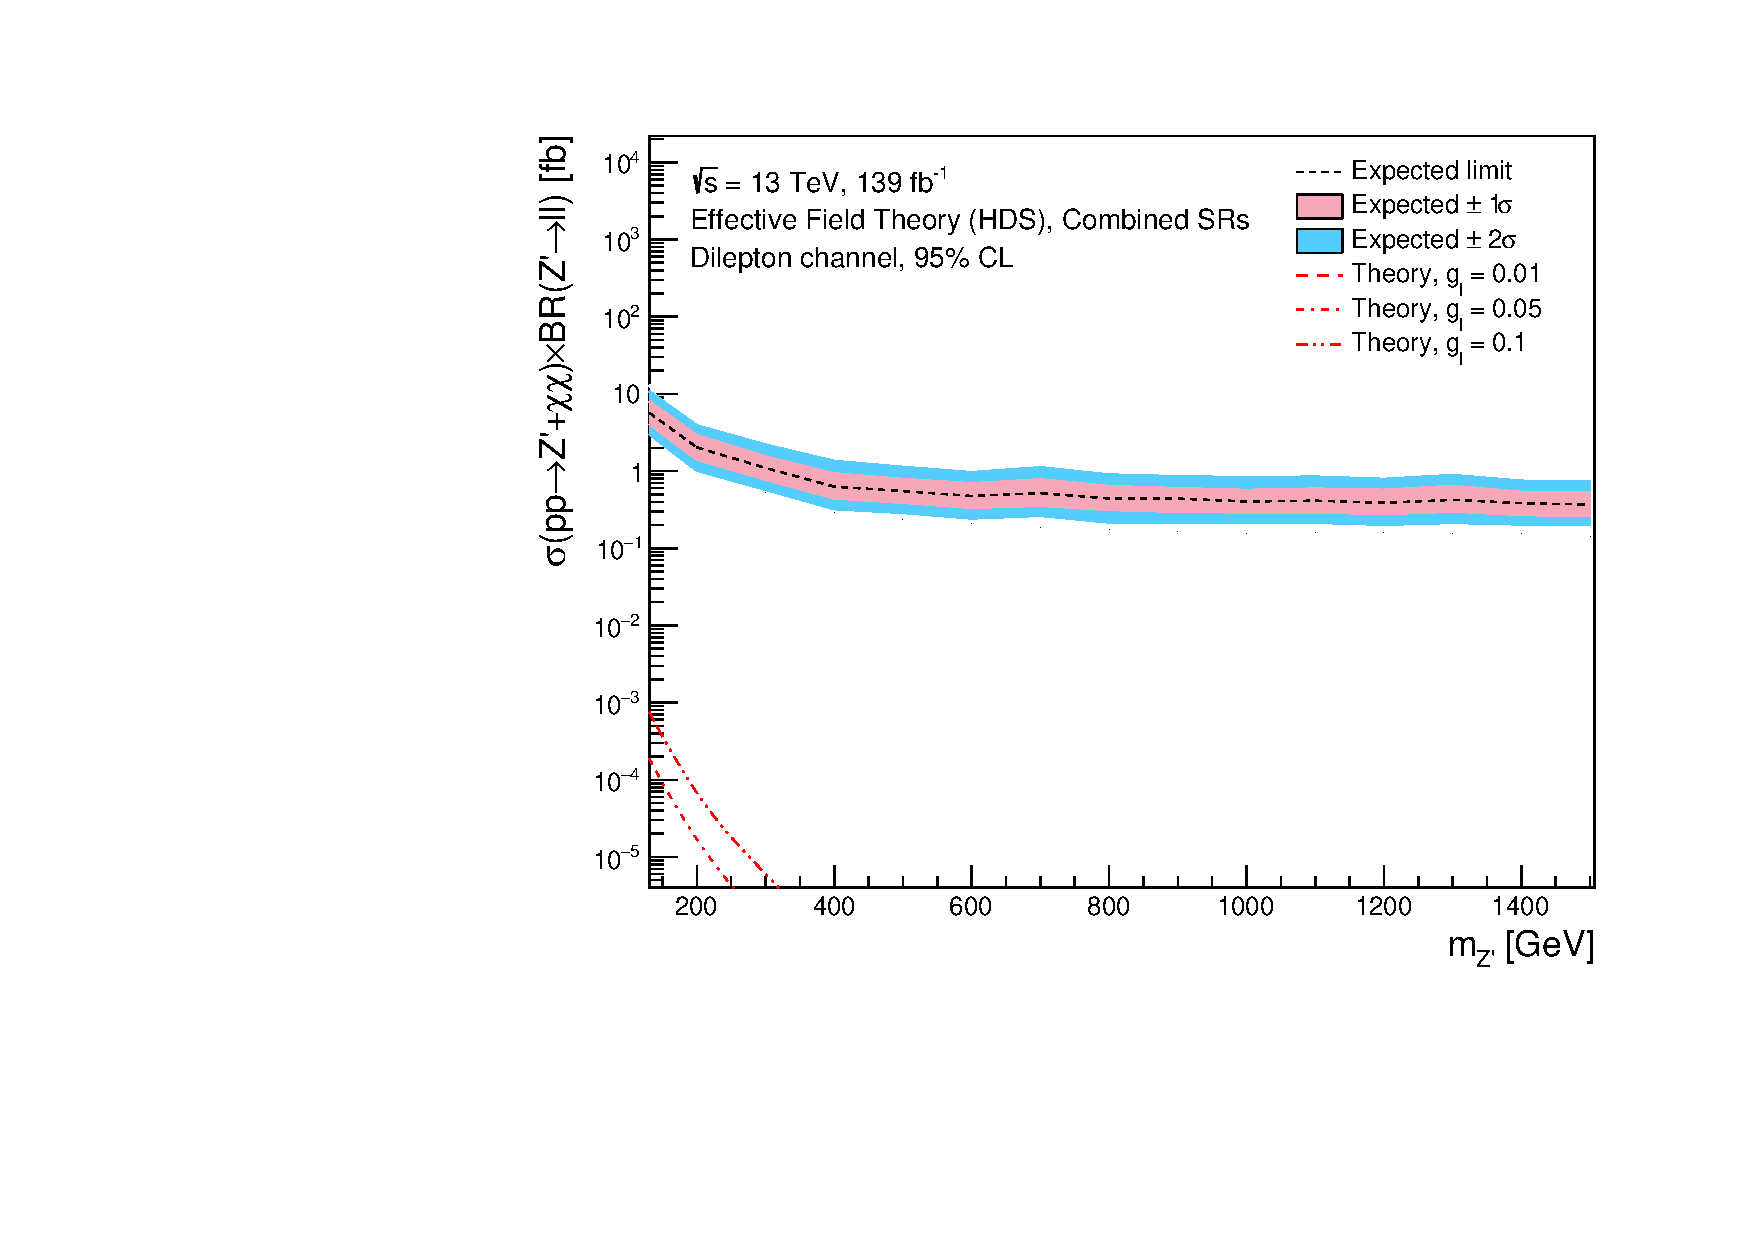
\includegraphics[width=1\textwidth]{Limits/Model_independent/EFT_HDS/mass_exclusion_comb.pdf}
   \end{subfigure}
   \hfill
   \begin{subfigure}[b]{0.49\textwidth}
      \centering
      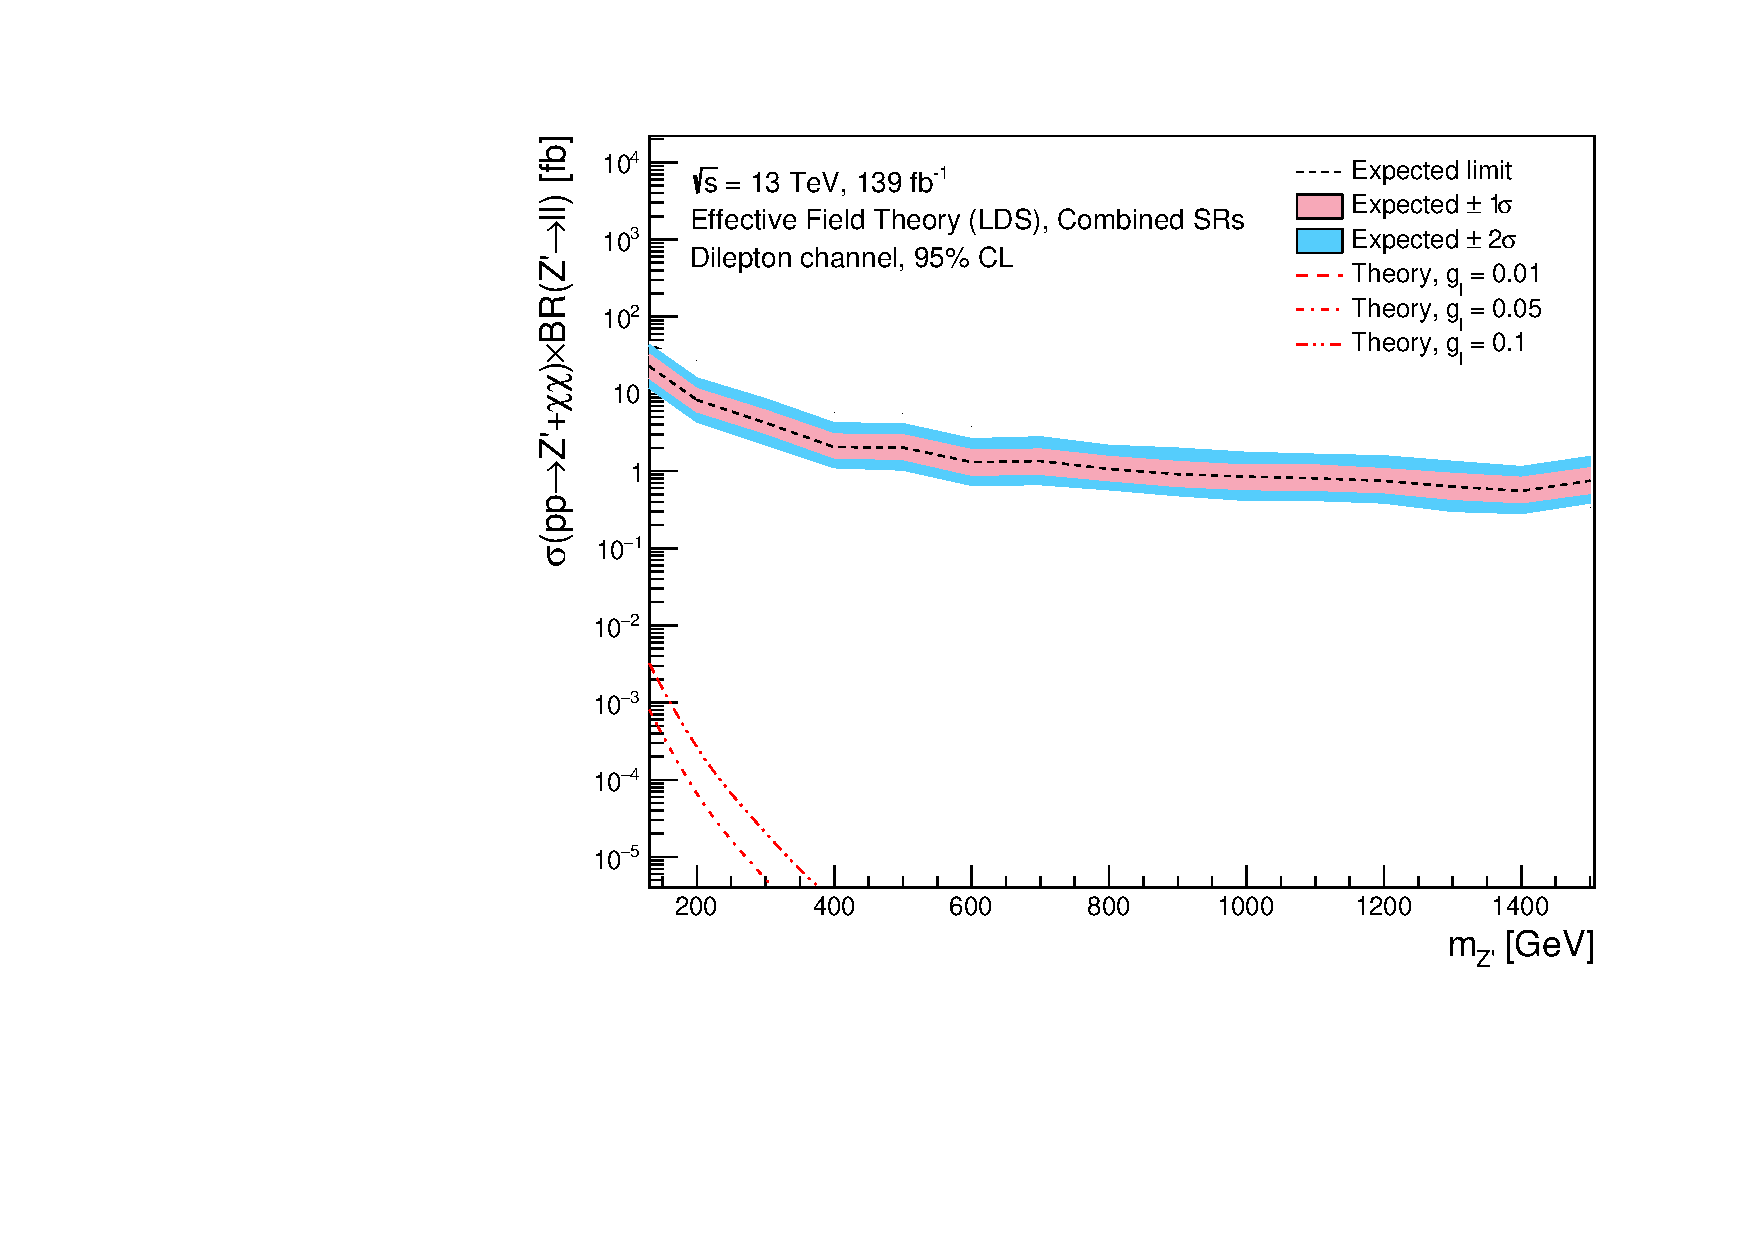
\includegraphics[width=1\textwidth]{Limits/Model_independent/EFT_LDS/mass_exclusion_comb.pdf}
   \end{subfigure}
   \caption[Mass exclusion limits of combined $ee$ and $\mu\mu$ channel for all mono-$Z'$]{Mass exclusion limits of combined $ee$ and $\mu\mu$ channel for all mono-$Z'$ models}
\end{figure}


\begin{figure}[!ht]
	\centering
	\begin{subfigure}[b]{0.49\textwidth}
      \centering
      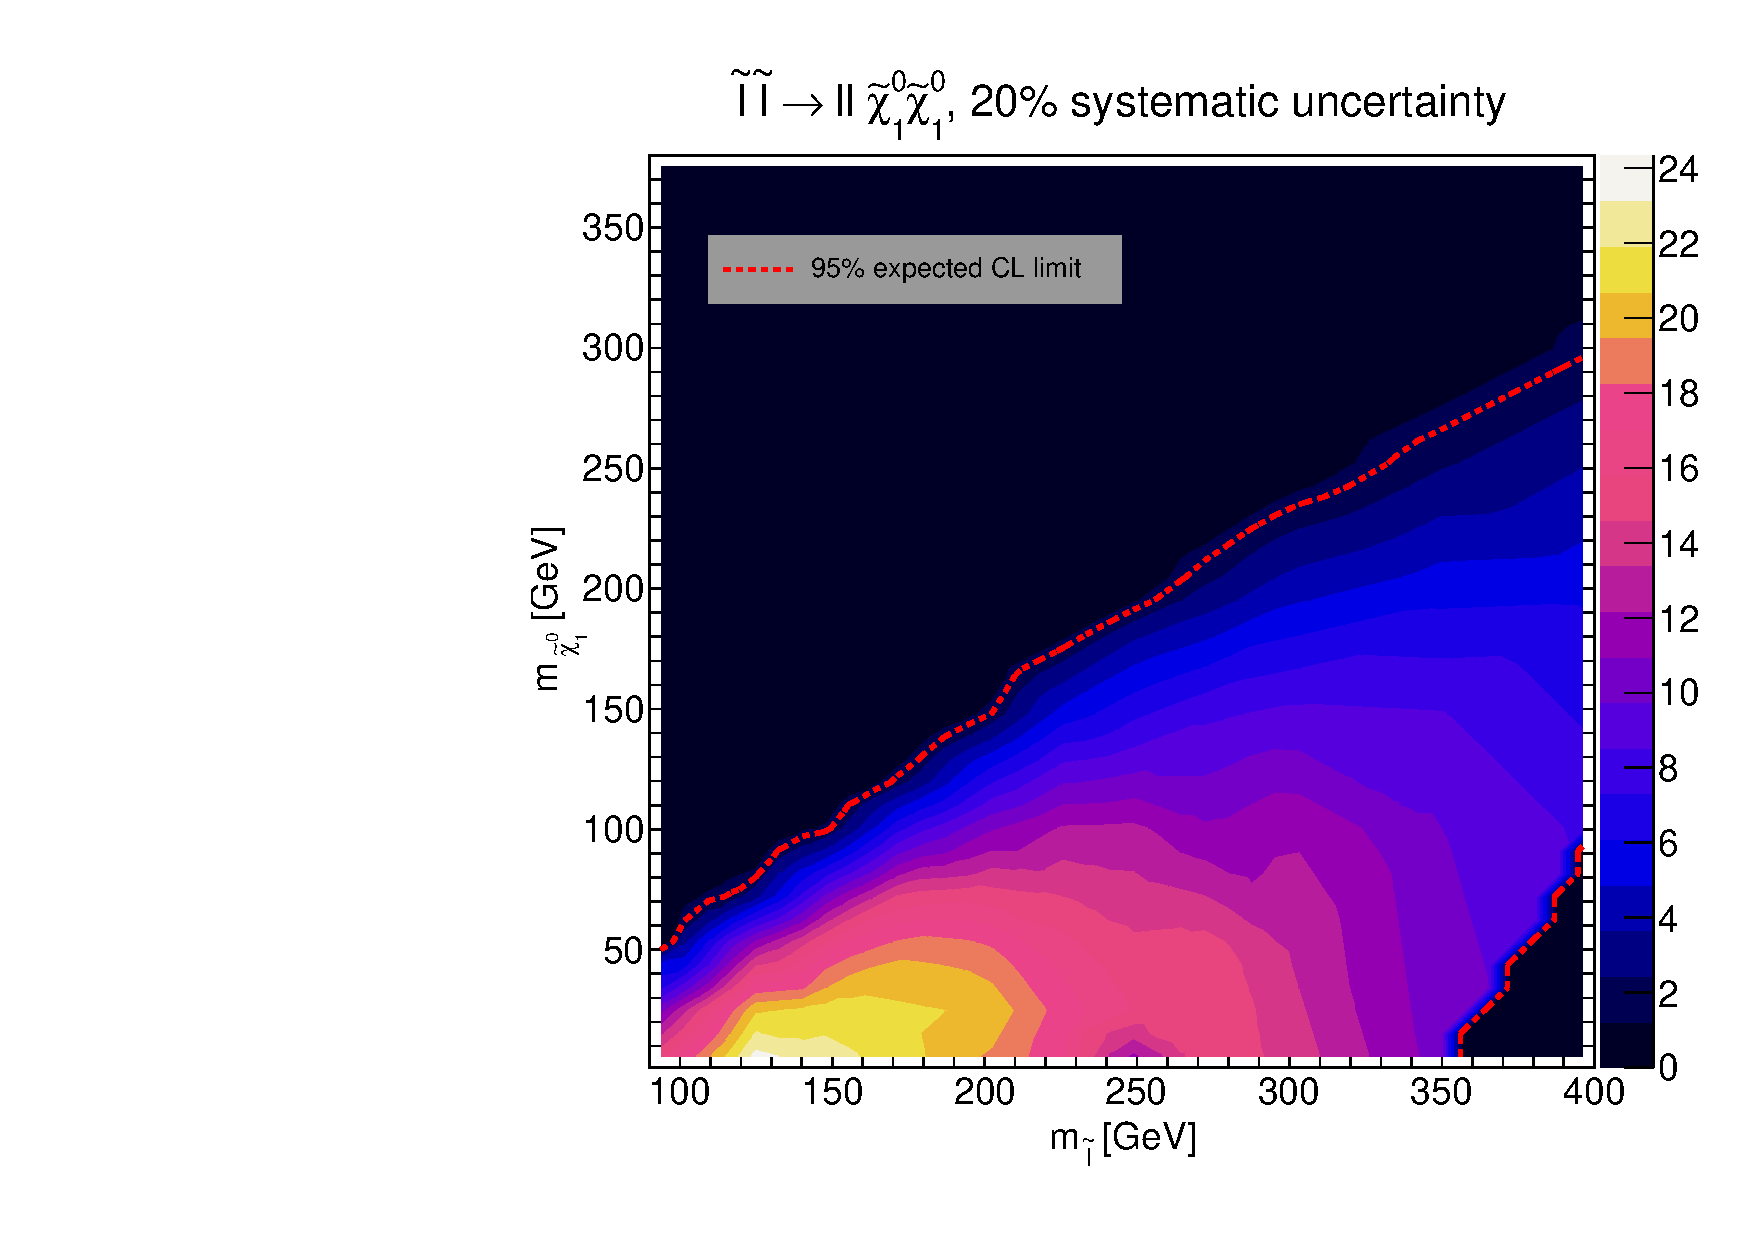
\includegraphics[width=1\textwidth]{Limits/Model_independent/SlepSlep/SlepSlep_ll.pdf}
   \end{subfigure}
   \hfill
   \begin{subfigure}[b]{0.49\textwidth}
      \centering
      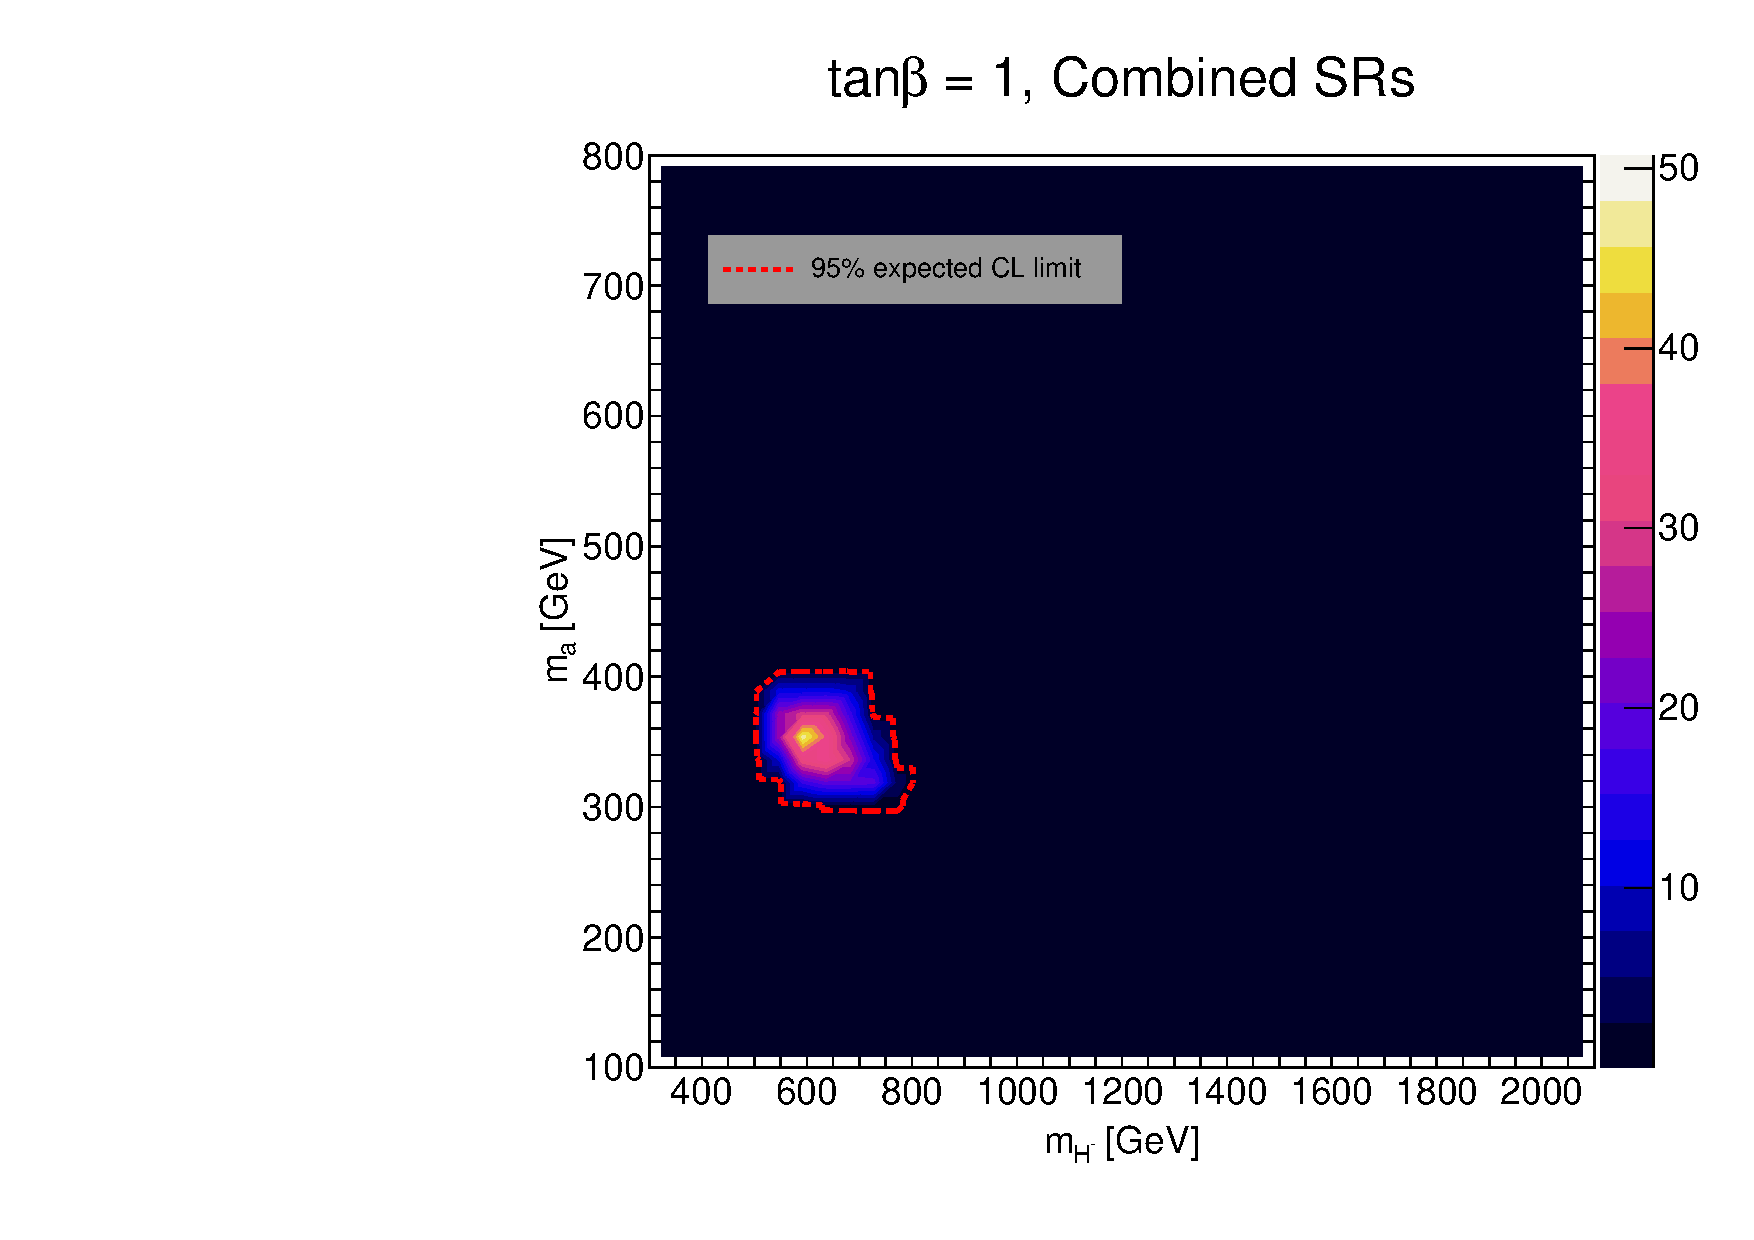
\includegraphics[width=1\textwidth]{Limits/Model_independent/2HDM/2HDM_ll_tb1.pdf}
   \end{subfigure}
   \hfill
   \begin{subfigure}[b]{0.49\textwidth}
      \centering
      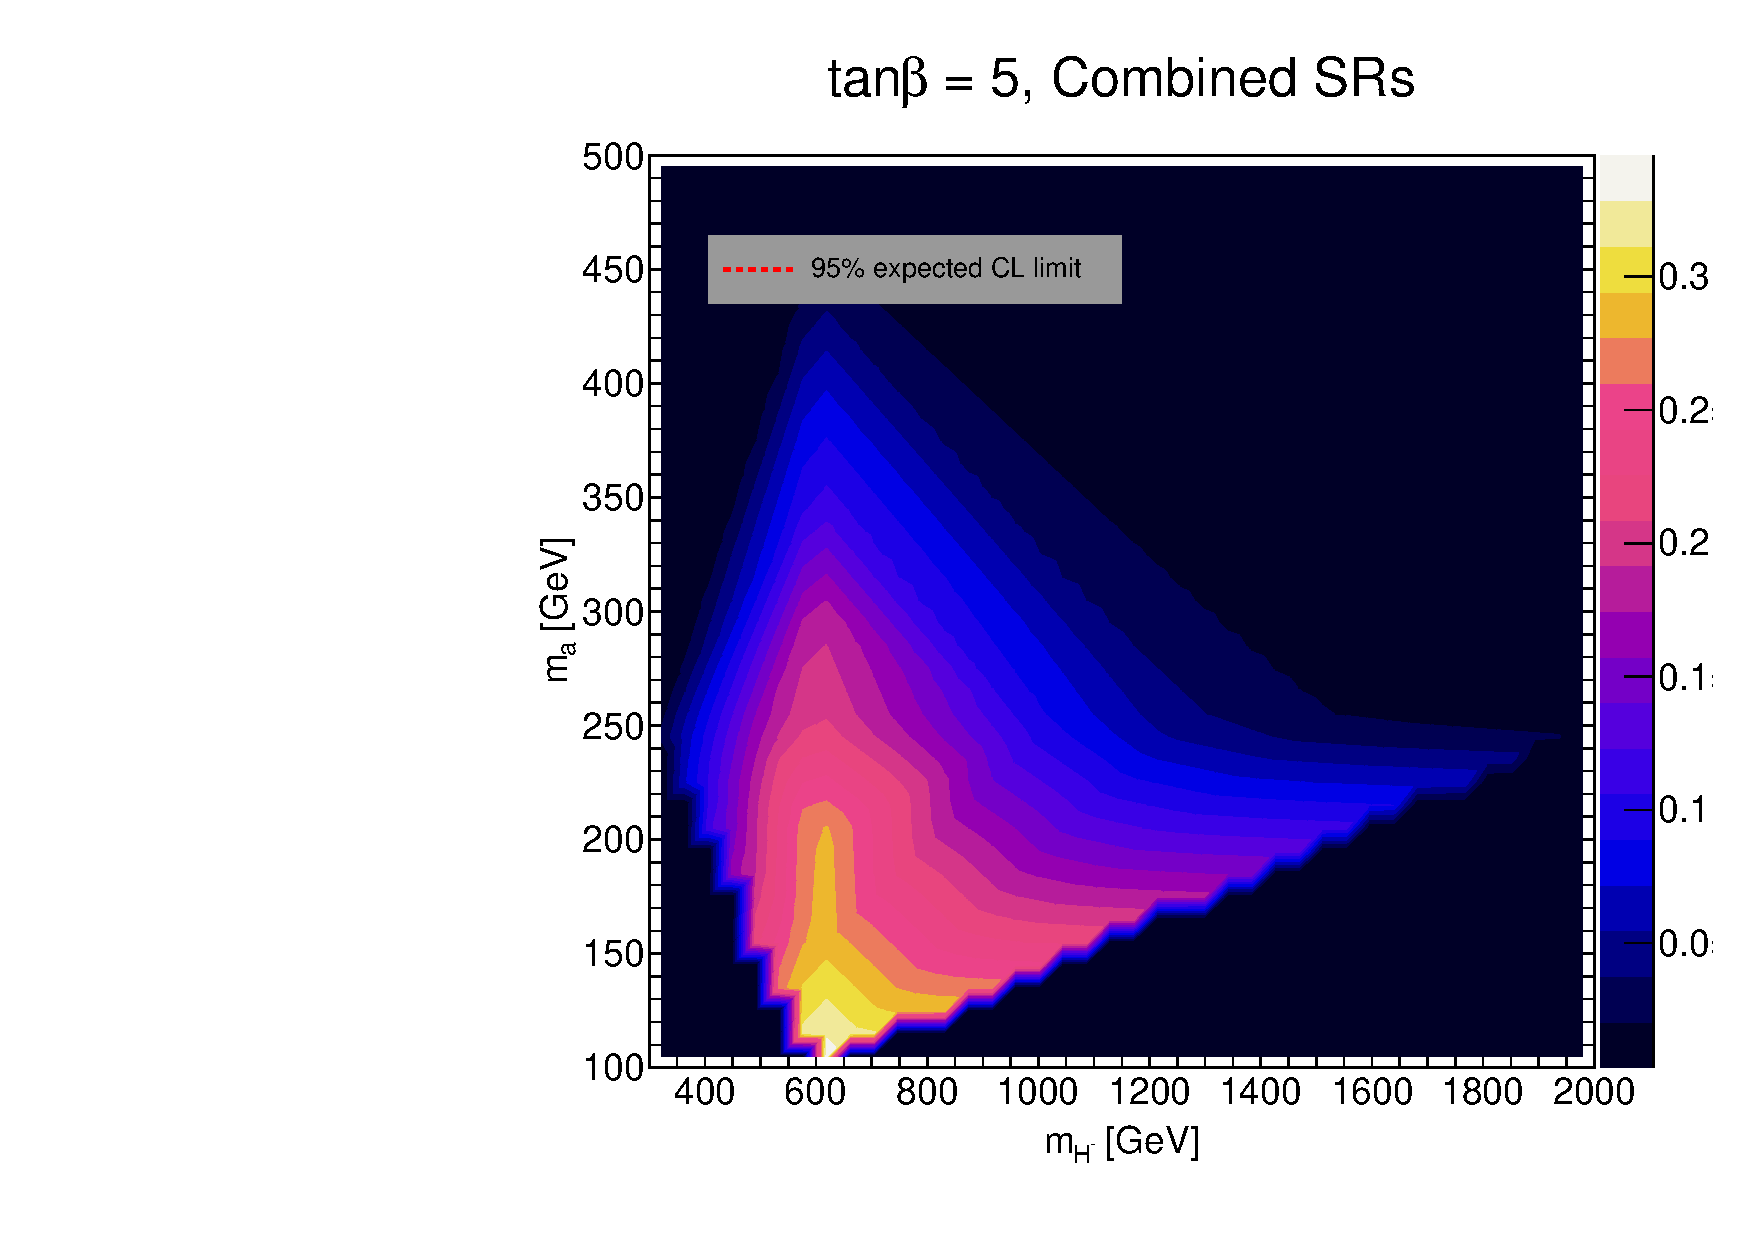
\includegraphics[width=1\textwidth]{Limits/Model_independent/2HDM/2HDM_ll_tb5.pdf}
   \end{subfigure}
   \hfill
   \begin{subfigure}[b]{0.49\textwidth}
      \centering
      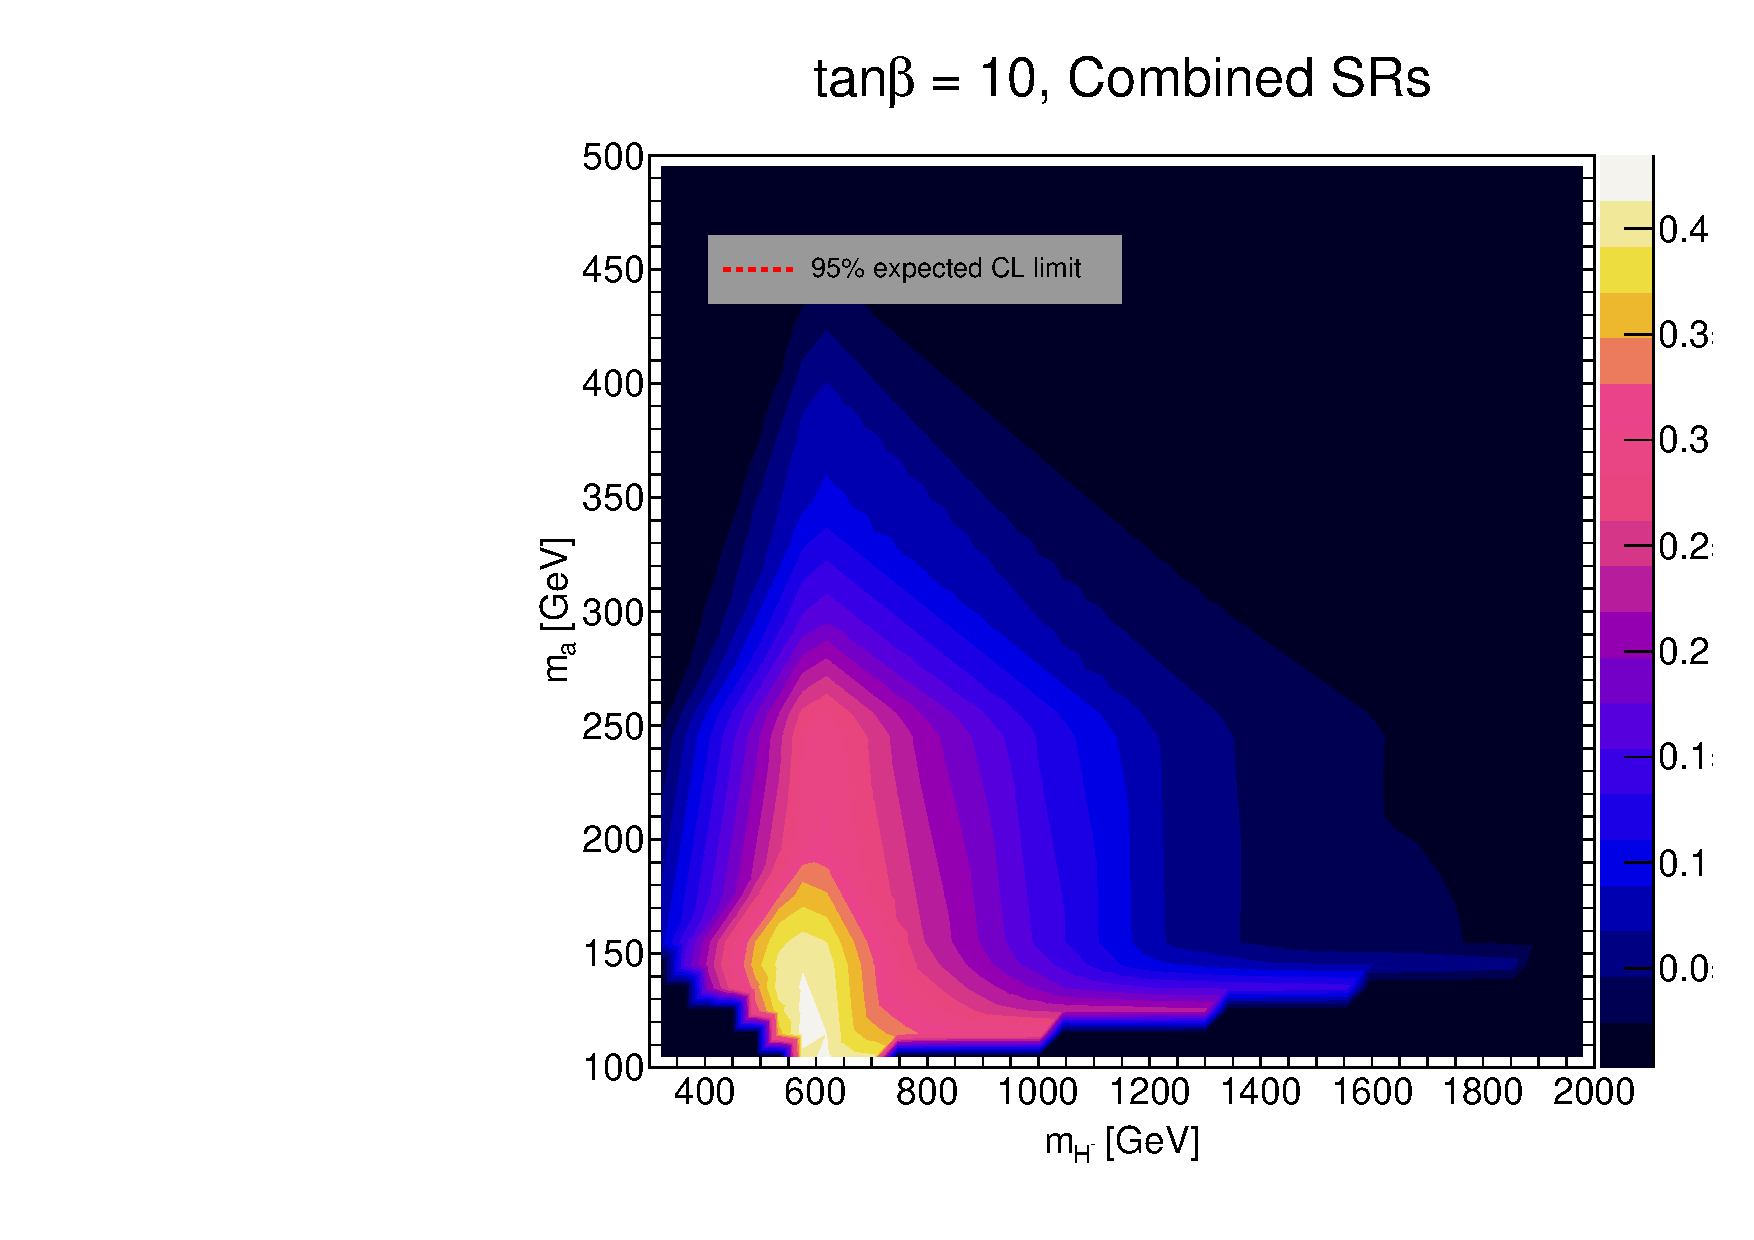
\includegraphics[width=1\textwidth]{Limits/Model_independent/2HDM/2HDM_ll_tb10.pdf}
   \end{subfigure}
   \hfill
	\begin{subfigure}[b]{0.49\textwidth}
      \centering
      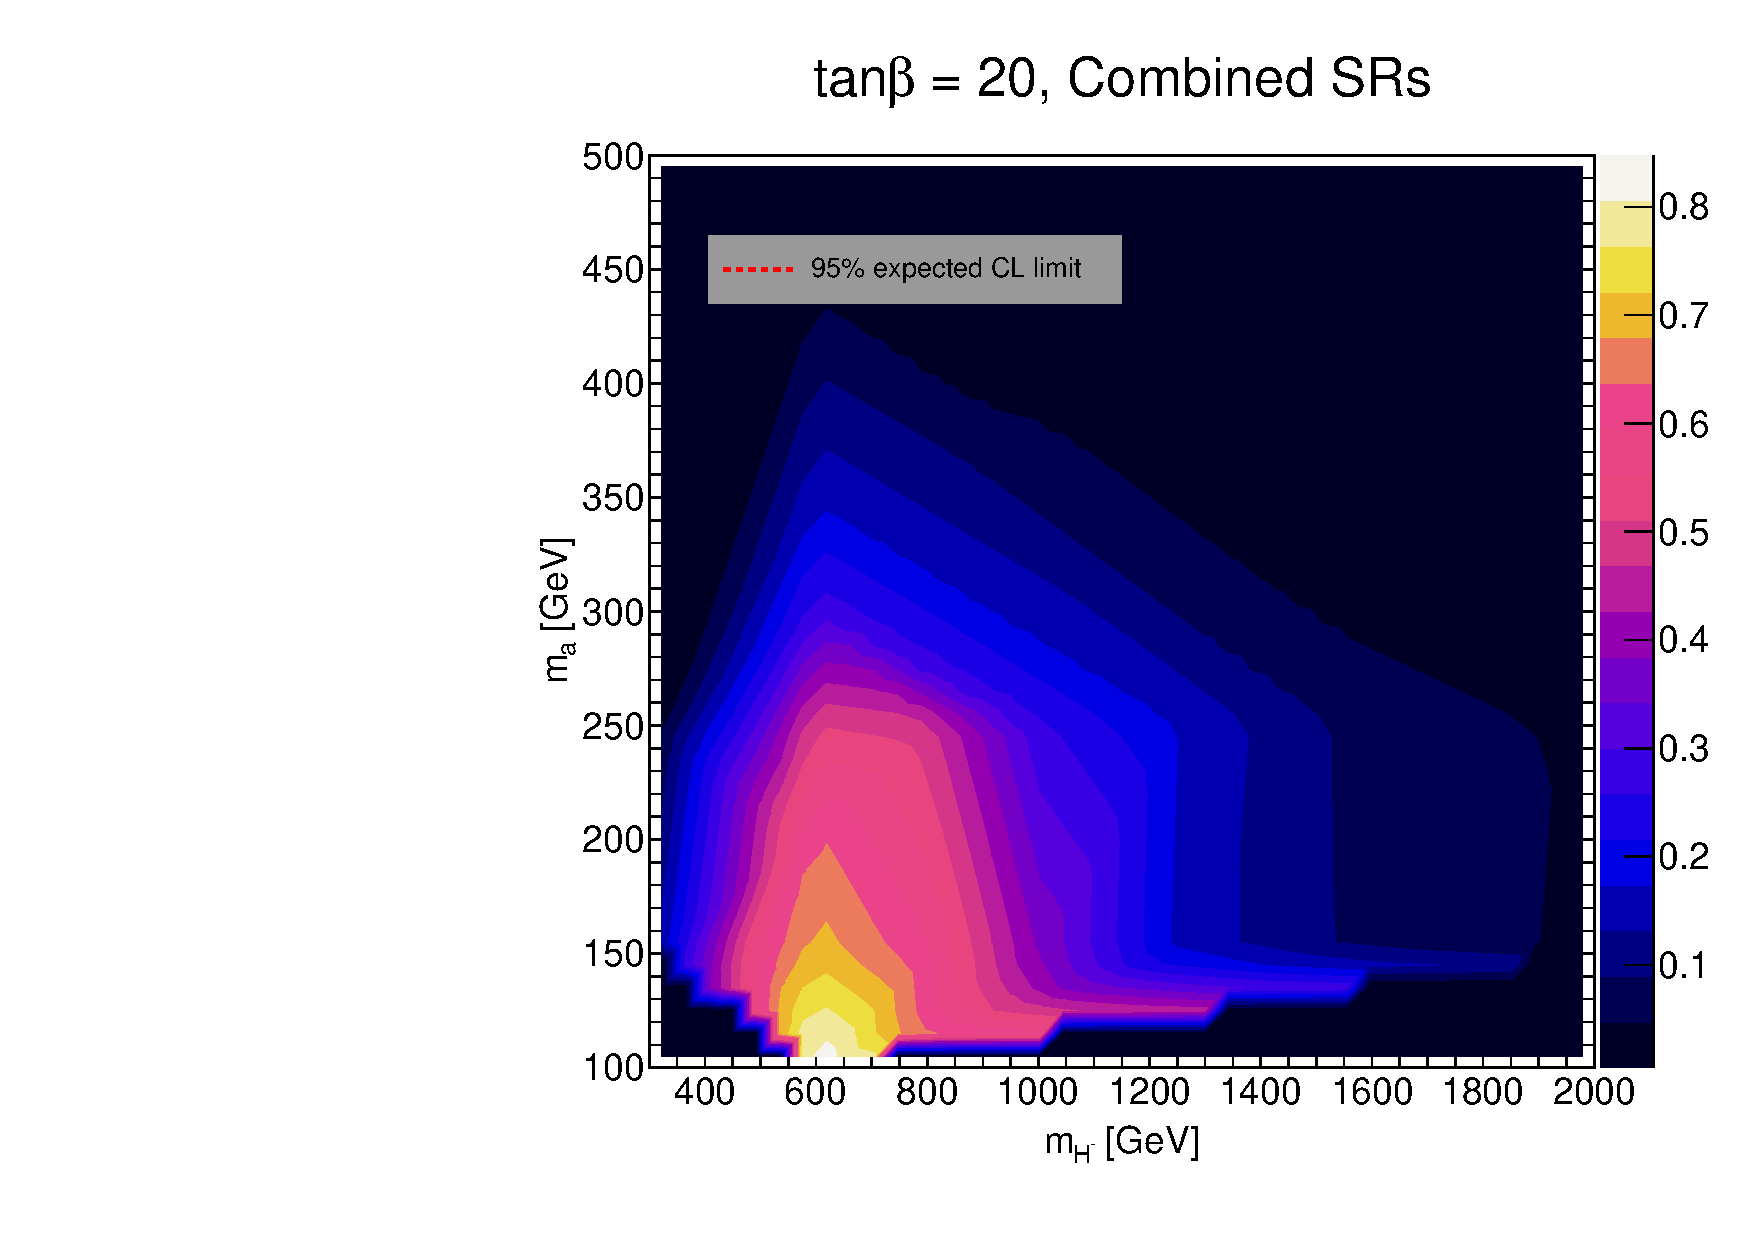
\includegraphics[width=1\textwidth]{Limits/Model_independent/2HDM/2HDM_ll_tb20.pdf}
   \end{subfigure}
   \hfill
   \begin{subfigure}[b]{0.49\textwidth}
      \centering
      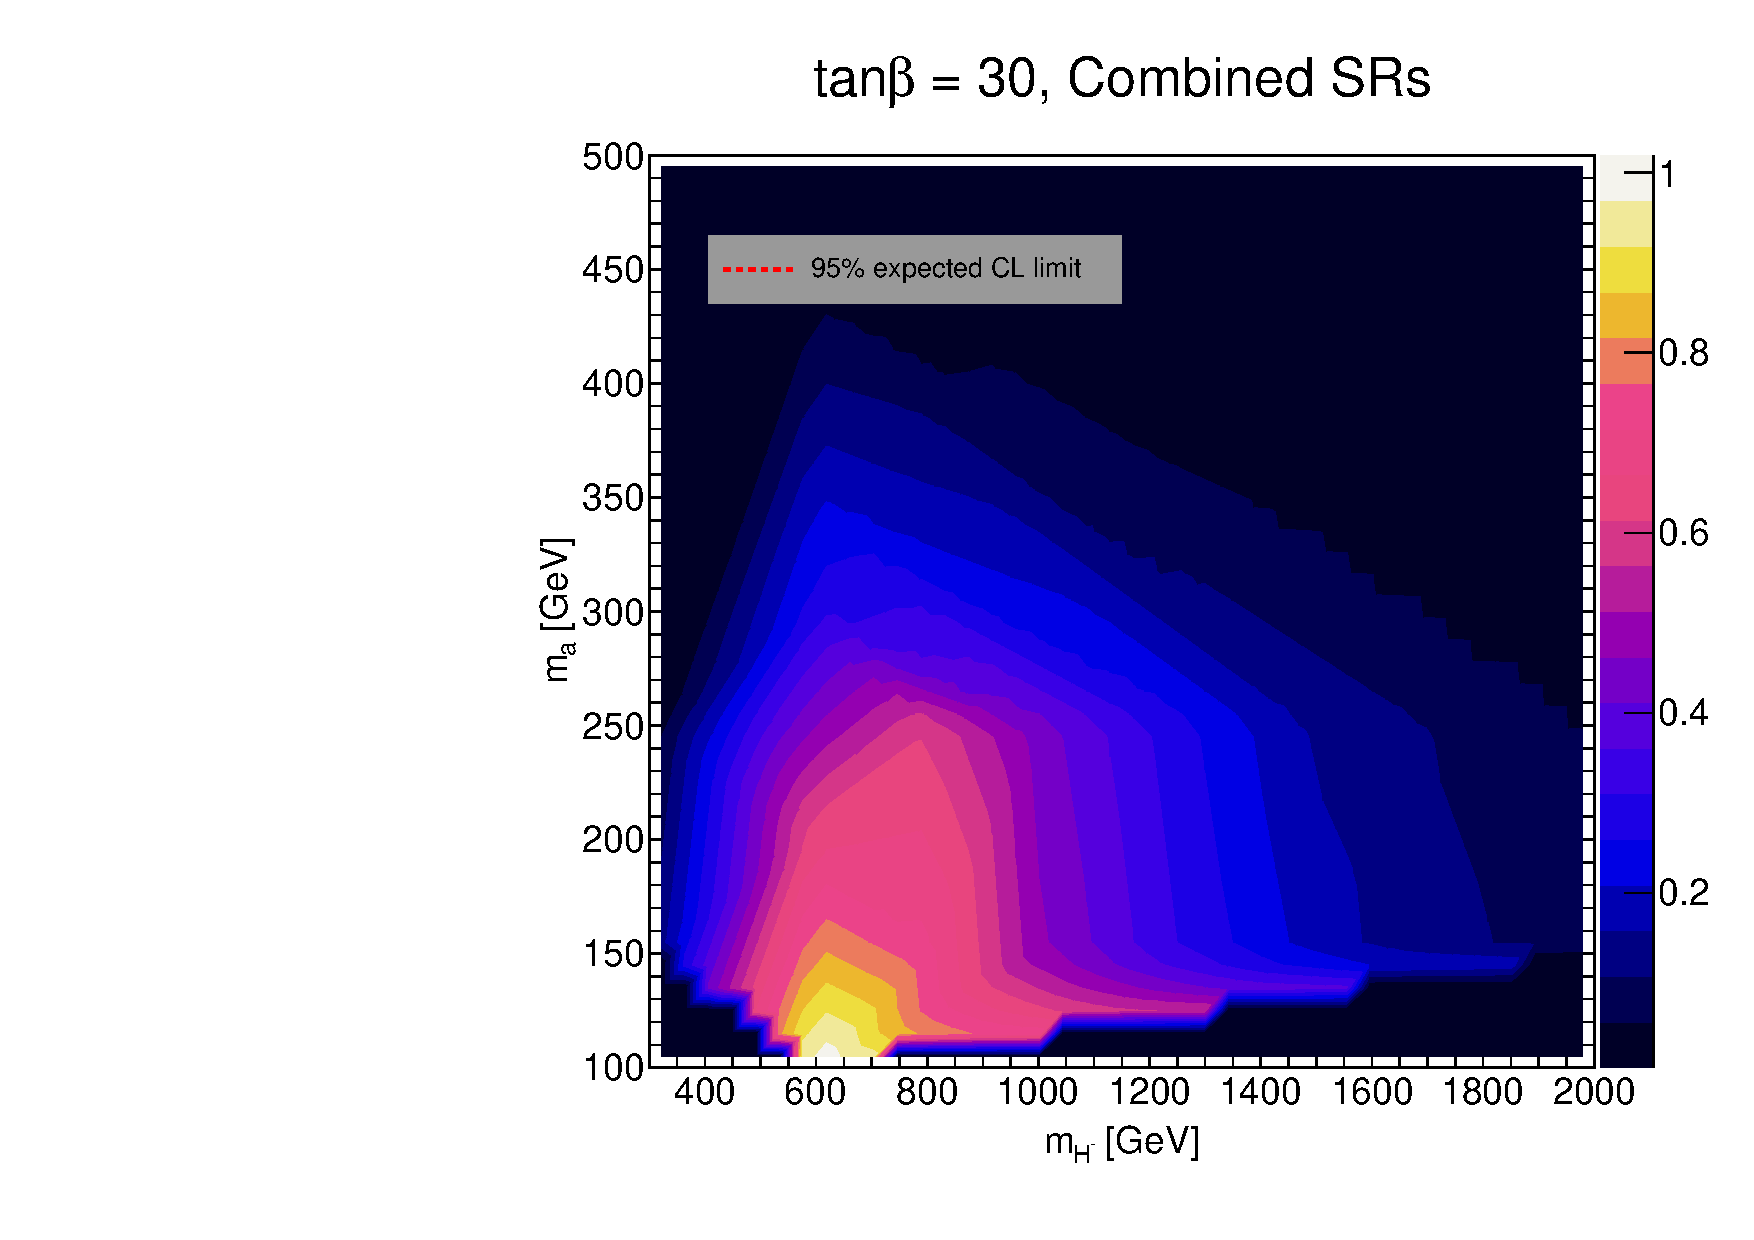
\includegraphics[width=1\textwidth]{Limits/Model_independent/2HDM/2HDM_ll_tb30.pdf}
   \end{subfigure}
   \caption[Mass exclusion limits of combined $ee$ and $\mu\mu$ channel for all mono-$Z'$]{Mass exclusion limits of combined $ee$ and $\mu\mu$ channel for all mono-$Z'$ models}
\end{figure}


\clearpage
\end{document}